%%
%% Copyright 2007, 2008, 2009 Elsevier Ltd
%%
%% Template article for Elsevier's document class `elsarticle'
%% with numbered style bibliographic references
%% SP 2008/03/01
%%
\documentclass[preprint,12pt,3p]{elsarticle}

\usepackage{rotating}
\usepackage{subfig}
%% The amssymb package provides various useful mathematical symbols
\usepackage{amssymb}
\usepackage{amsmath}
%% The amsthm package provides extended theorem environments
\usepackage{amsthm}
\usepackage{times} % assumes new font selection scheme installed
\usepackage{graphics} % for pdf, bitmapped graphics files
\usepackage{float}
\usepackage{xcolor}
\definecolor{verde}{rgb}{0,0.5,0}


\usepackage{fancyhdr}
\pagestyle{fancy}
\fancyhf{}
\renewcommand{\sectionmark}[1]{\markboth{\thesection. #1}{}}
\renewcommand{\subsectionmark}[1]{\markright{\thesubsection. #1}}
\fancyhead[L]{%
  \leftmark
}
\fancyhead[R]{\rightmark}
\renewcommand{\headrulewidth}{1pt}
\renewcommand{\headrule}{\hbox to\headwidth{%
  \color{verde}\leaders\hrule height \headrulewidth\hfill}}

\usepackage[colorlinks,citecolor=blue,urlcolor=blue]{hyperref}
\usepackage{cleveref}
\usepackage{listings}
\lstset{
    %frame=tb, % draw a frame at the top and bottom of the code block
    tabsize=4, % tab space width
    showstringspaces=false, % don't mark spaces in strings
    numbers=left, % display line numbers on the left
    %commentstyle=\color{verde}, % comment color
    %keywordstyle=\color{blue}, % keyword color
    %stringstyle=\color{red} % string color
	belowcaptionskip=1\baselineskip,
	breaklines=true,
	frame=false,
	xleftmargin=\parindent,
	basicstyle=\scriptsize\ttfamily,
	%basicstyle=\footnotesize\ttfamily, %edit to get bigger font
	keywordstyle=\bfseries\color{green!40!black},
	commentstyle=\itshape\color{purple!40!black},
	identifierstyle=\color{blue}, %functions
	stringstyle=\color{orange},
}
\lstnewenvironment{ttlisting}{\lstset{ 
	basicstyle=\scriptsize\ttfamily\color{black}, identifierstyle=\color{darkgray},}}{}
%% The lineno packages adds line numbers. Start line numbering with
%% \begin{linenumbers}, end it with \end{linenumbers}. Or switch it on
%% for the whole article with \linenumbers after \end{frontmatter}.
\usepackage{lineno}

%% natbib.sty is loaded by default. However, natbib options can be
%% provided with \biboptions{...} command. Following options are
%% valid:

%%   round  -  round parentheses are used (default)
%%   square -  square brackets are used   [option]
%%   curly  -  curly braces are used      {option}
%%   angle  -  angle brackets are used    <option>
%%   semicolon  -  multiple citations separated by semi-colon
%%   colon  - same as semicolon, an earlier confusion
%%   comma  -  separated by comma
%%   numbers-  selects numerical citations
%%   super  -  numerical citations as superscripts
%%   sort   -  sorts multiple citations according to order in ref. list
%%   sort&compress   -  like sort, but also compresses numerical citations
%%   compress - compresses without sorting
%%
%% \biboptions{comma,round}

% \biboptions{}


\journal{Final report for Spring 2018 rotation in Harvard Biorobotics Lab}
\begin{document}

\begin{frontmatter}

\title{ Improving end joint sensing for robotic grasping\\
(Using IMUs to estimate contact force) }

%\tnotetext[label0]{This is only an example}

\author{Nao Ouyang}
%\address[label1]{Address One}

%\address[label2]{Address Two\fnref{label4}}
%\author[label1,label2]{Author One\corref{cor1}\fnref{label3}}
%\address[label1]{Address One}
%\address[label2]{Address Two\fnref{label4}}

%\cortext[cor1]{I am corresponding author}
%\fntext[label3]{I also want to inform about\ldots}
%\fntext[label4]{Small city}

%\ead{author.one@mail.com}
%\ead[url]{author-one-homepage.com}

%\author[label5]{Author Two}
%\address[label5]{Some University}
%\ead{author.two@mail.com}

%\author[label1,label5]{Author Three}
%\ead{author.three@mail.com}

\begin{abstract}
    Despite decades of research, robots remain unable to reliably grasp objects in environments not
    designed for robots. Thus, they are not able to work alongside us in human environments or
    outside buildings. One approach is to use tactile sensing to predict whether a
    grasp will succeed or not as well as build simulations to evaluate potential grasps.
    In this lab, we use an underactuated three-fingered gripper, which makes it difficult to
    estimate the location of the fingers and and the location of the force with respect to the robot
    frame of reference.  \\
    I investigated the use of an inertial measurement unit to provide such information. By
    characterizing the stiffness matrix $K$ of the finger, I could investigate whether using an
    inexpensive inertial measurement unit (IMU) to estimate $\theta$ deflection with the linear equation
    $\tau = K \theta$, I could discover information about the force applied. I did very preliminary
    work, limiting my experiments to the case where we only desire to estimate the change from
    directly before to second or two after
    contact. I also I looked at using of off-the-shelf machine learning approaches to reduce the
    errors in our model. Finally, I investigated adding more sensors to the fingertip in
    order to better estimate contact location. 
\end{abstract}



\end{frontmatter}

%%
%% Start line numbering here if you want
%%
% \linenumbers

%% main text


\section{Introduction}
State-of-the art robots are bad at grasping in unstructured environmnents, limiting their use to
structured environments like factory floors. An active area of research in order for robots to expand to unstructured
environments (such as kitchens or hospital environments),  is the ability to grasp
novel objects (objects the robot has not encountered before and may not have any prior information
about). Grasp stability analysis plays a critical role in enabling robots to achieve high grasping
success rates (in terms of not dropping objects). Through sensing, for instance tactile sensing, we
can predict whether or not we will drop the object after grasping and prior to moving. If we find
our grasp to be unstable, and assuming the object has not moved during grasping such that releasing
our grip might e.g. cause it to tumble, we can simply release our grasp and try again. 

Physical model approaches involve modeling the contact forces, contact location, and surface normals
(which will differ from the force XYZ if the surface(s) are squishy).  However, over the last few
decades physical models have proven insufficient. This in part due to complex gripper-object
interactions during grasping which are both difficult to measure and hard to model. Thus, one of the
aspects of this investigation is to evaluate whether machine learning can be used to improve
physical models. We can combine the good aspects of physical models (good generalizability,
requiring significantly less data than in pure computer vision machine learning approaches) with
(not having to have extremely precise models). I tried to charactize the residuals in
the physical models and determine if these residuals could be more accurately modelled by a black
box machine learning approach rather than making the physical model more complex. This is an
increasingly popular approach, which makes intuitive sense. We can leverage
domain knowledge, instead of using an end-to-end approach for sensor data to stability prediciton.

Although there are a few compact 6 axis force torque sensors, they cost multiple thousands of
dollars and are finicky and fragile. Thus, we would like to use an inexpensive nine
degree-of-freedom (three-axis acceleromter, gyrometer, and magnetic heading) IMU instead.

During the course of this rotation, senior graduate student Qian Wan discoverd that the current tactile
sensors are insufficent for estimating contact location accurately enough to develop a good grasp
stability estimate. Thus, this project includes a brief exploration of a new sensor design using the
same elements (barometric pressure sensors covered by a layer of elastomer, such as urethane), but
more of them.

\section{Theory} \label{sec:firstpage}

\subsection{Linear Model}

For the physical model, I am making a few simplifying assumptions:
 
    \begin{enumerate}
        \item There is a linear relationship between force and deflection, or alternatively torque and angle of deflection
        \item The center of the axis of rotation was at the tip of the proximal joint
    (in reality, likely it is two or three mm shifted outward, and changes as the flex increases)
        \item We consider the z axis to be defined respect to the surface of the finger, so that z=0 is always
    at the tip of the finger
    \end{enumerate}

Note that the consequence of \#3 is that we cannot estimate z-axis torque.

\subsection{Reference Frame}

\begin{ttlisting}[language=C++,breaklines]
Coordinates
----> + x (roll)
|
|
v
+ y (pitch)

+ z (up out of page) (yaw)


Finger Positions
=======      ====================.
 {CL}  || --- || 15  12  9  6  3 ||
 {A} [xy=0]-- || 14  11  8  5  2 ||
 {MP}  || --- || 13  10  7  4  1 ||
=======      ====================.


  [[---]]
||  WEB  ||
||  CAM  ||
  ||--- ||
  
\end{ttlisting}

For the initial (3D stiffness matrix) experiment, Points 13 through 15 are at x=2.6 cm, and each x is spaced 5 mm apart.
The y's are at 0.4, 0.1, and -0.2mm respectively.

For the final experiment comparing two stiffness, the x spacing remains roughly the same, while the
y's are now at 0.3, -0.1, and -0.4 mm respectively.
~\\

\subsection{Linear Model in the 1D case}

In the one-axis case, the math is straightforward. Experimentally, this is when I am only collecting
data down the center (y-axis) of the finger, which should result in almost no roll and pitch,
limiting the analysis to yaw. 

\begin{align}
\tau = k \times F
\end{align}

For example, one datapoint might be

\begin{align}
k &= F / \tau \\
k &= (20g \times 9.8 m/s^2)/0.1 \text{ degrees}
\end{align}

where `k` represents the stiffness of the finger. Let $c$ represent the inverse of $k$.

Using least squares error, we may fit a line to find $\hat{c}$. 

\begin{align}
 \hat{c} &= \frac{1}{\hat{k}} \\
 \theta &= \tau \hat{c} + b
\end{align}

where $b$ be a constant determined by the line of fit.



\subsection{Linear model residuals}

From the above, we may calculate the residuals of any of our estimated variables.
For instance, from our actual data we may obtain an estimate for `k`.

\begin{align}
 \tau_{data} &= \hat{k} \cdot \theta_{data} \\
\end{align}

Using this k we can go back and calculate estimates for the "true" torque, assuming our linear model was correct.

\begin{align}
 \hat{\tau} &= \hat{k} \cdot \theta_{data} 
\end{align}

We would then calculate our torque residuals as

\begin{align}
 \epsilon_{\tau} = \hat{\tau} - \tau 
\end{align}

If we plot a graph of (torque residuals) vs (estimate residuals) and find that our points are randomly scattered around a straight line, then our model well-approximates reality as sensed by a noisy sensor.

However, our residuals may instead follow a parabola, in which case we would want to amend our model
to have higher-order terms.

\begin{align}
 \hat{\tau} = \hat{k}\theta_{data} +c_1 \theta_{data} + c_2 \theta_{data}
\end{align}

and so forth. 

We may eventually use machine learning techniques to fit higher-order terms.

\subsection{Linear model in the 3D case}
\label{3d case}
The 3d case is exactly the same, except now each of the variables are vectors or matrices. 

    %:s@\\\[:\\begin{bmatrix}:g
\begin{align}
    \begin{bmatrix} \vec{\tau} \end{bmatrix}_{3\times n}  = \begin{bmatrix} K \end{bmatrix}_{3\times 3} \cdot \begin{bmatrix} \vec{\theta} \end{bmatrix}_{3\times n} 
\end{align}

where

\begin{align}
\vec{\tau} &= \begin{bmatrix} \stackrel{3\times 1}{\tau_1} | \stackrel{3\times 1}{\tau_2} | ... |\stackrel{3\times 1}{\tau_n} \end{bmatrix} \\
\\
\vec{\theta} &= \begin{bmatrix} \stackrel{3\times 1}{\theta_1} | \stackrel{3\times 1}{\theta_2} | ... |\stackrel{3\times 1}{\theta_n} \end{bmatrix}
\end{align}

\subsection{Sanity Check: Simplify to 2D case}

We know that $\tau = r \times F$

\begin{align}
    \begin{bmatrix}
        \tau_{x} \
        \tau_{y} \
        \tau_{z} \
    \end{bmatrix} =
    \Bigg[ \; K \; \Bigg]_{3\times3} \;
    \begin{bmatrix}
        \theta_{x} \
        \theta_{y} \
        \theta_{z} \
    \end{bmatrix} \
\end{align}

Further, we can use some of the simplifying assumptions we made about to model our system, in order to have an idea of what values our math should result in for $k$.

We may also see that we will only ever have x and y components for $r$; z components for $F$; and thereforce (by how cross products work) only ever have x and y components for $\tau$.

\textbf{Off-axis}
\begin{align}
r \approx
\begin{bmatrix}
    r_x       \\
    r_y       \\
    0       \\
\end{bmatrix} \; \times \;
f \approx
\begin{bmatrix}
    0       \\
    0       \\
    f_z      \\
\end{bmatrix} \; =  \; \tau \; = 
\begin{bmatrix}
    \tau_x       \\
    \tau_y       \\
    0      \\
\end{bmatrix}\\
\end{align}


\textbf{On-Axis}

In the even more simplified case, if we do not apply the force off-axis and there is only a pitch
deflection

\begin{align}
r \approx
\begin{bmatrix}
    r_x       \\
    0       \\
    0       \\
\end{bmatrix} \; \times \;
f \approx
\begin{bmatrix}
    0       \\
    0       \\
    f_z      \\
\end{bmatrix} \; =  \; \tau \; = 
\begin{bmatrix}
    0 \\
    \tau_y       \\
    0      \\
\end{bmatrix}\\
\end{align}

We \textbf{could} have enough nonzero values for the xyz components of $\theta$ that we will be able
to calculate a nondegenerate estimate for $k$. This is thanks to applying the force off-axis,
causing the finger to roll and create non-zero elements for $\theta_y$ ( our roll) and $\theta_z$
(our yaw). However, after solving for K, I found that I ended up with a bottom row consisting
entirely of zeroes.


\section{Methods}

\subsection{Setup}

For the setup, I used a triple-beam balance as a way to apply force while retaining a vertical
angle. I hot-glued a pumpkin awl to the bottom of the plate and put standard weights on top of of
the scale. This caused the awl to contact the surface of the finger, and the finger would then
deflect. 

\begin{figure}[H]
\centering
%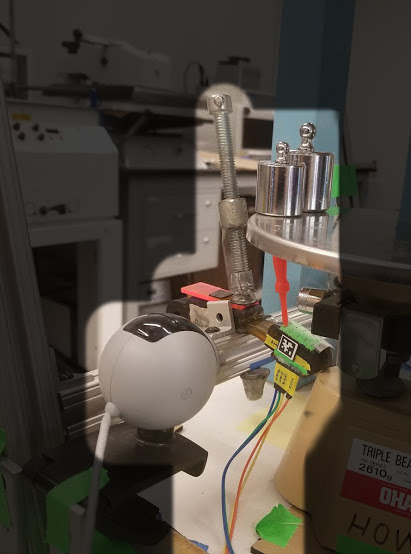
\includegraphics[width=.3\textheight]{images/setup/webcam-edit.jpg}
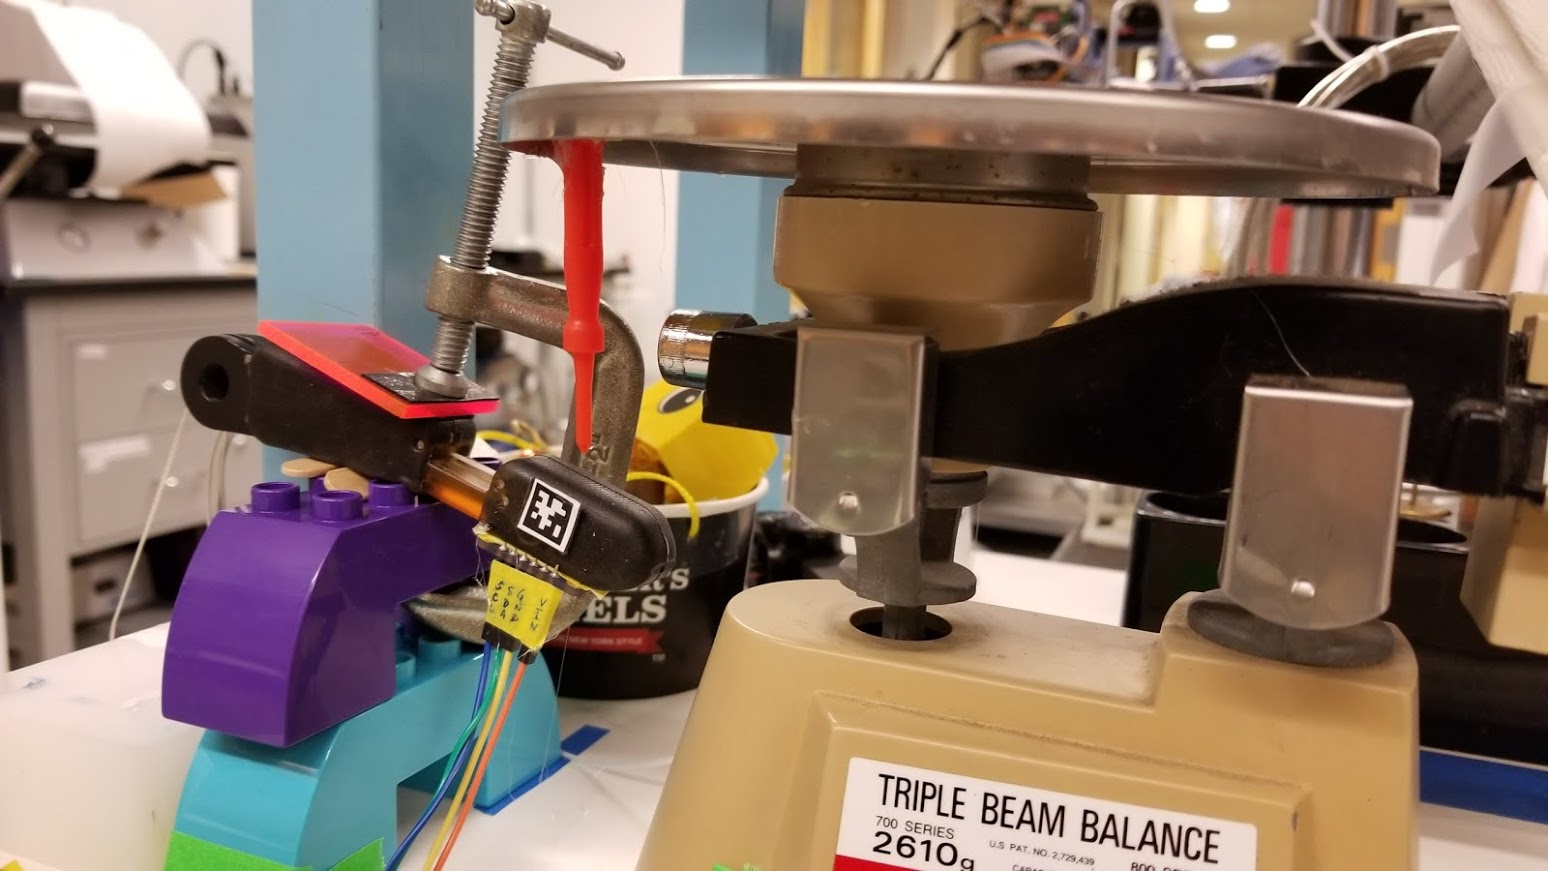
\includegraphics[width=.5\textheight]{images/setup/closeup.jpg}
%\caption{Loaded tendon}
%\label{fig:figura1}
\end{figure}


\subsubsection{One-Dimension Data}
In the 1D case, I simply placed a ruler behind the finger and used a webcam to take
pictures. By mapping pixel counts to millimeters, I could then estimate the deflection of the
finger. The linear fit from these very imprecise measurements proved linear enough that I then
relied on the IMU going forward and skipped the step (which should be completed eventually) of
characterizing the accuracy of the IMU versus a gold standard, such as a stereo camera (the
Microntracker available in lab) or other methods (such as using Apriltags with a calibrated webcam). 

In the 1D case I simply took pictures of the finger against a ruler in order to measure angular deflection. 

\begin{figure}[htbp]
    \centering 
        \subfloat[Zero measurement
        ]{%
            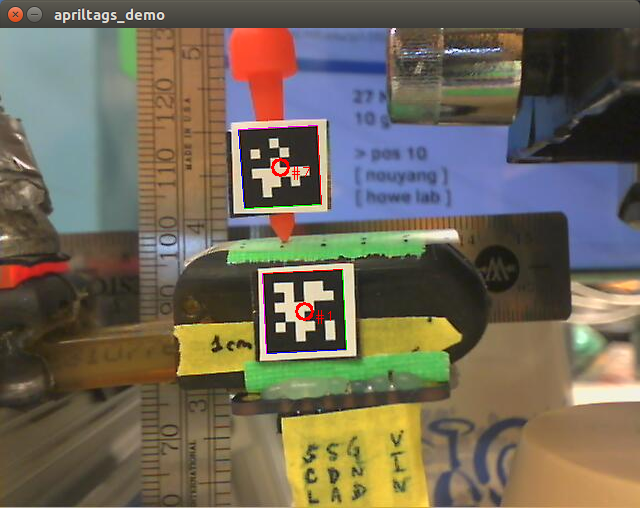
\includegraphics[width=0.3\linewidth]{images/1d/zero.png}%
        }\hfil % MUST be right above next figure
        \subfloat[Weight (torque) applied 
        ]{%
            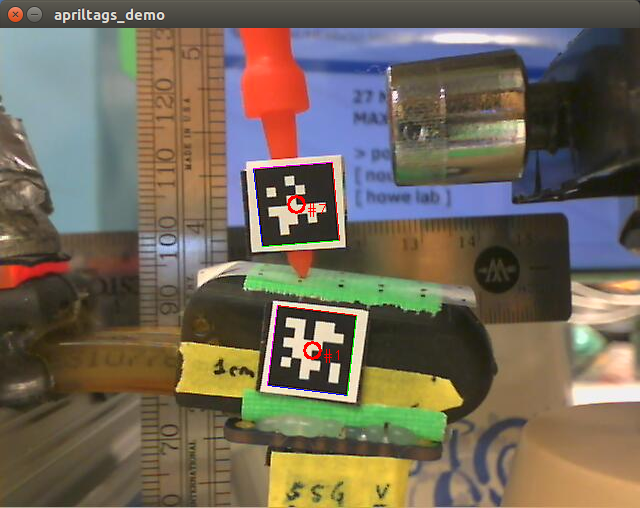
\includegraphics[width=0.3\linewidth]{images/1d/weighted.png}%
        }\hfil
        \caption{I drew lines through the vertical (with reference to the camera image) center of
            the finger before and after weight was applied. The angle between the two is what I
        wrote down}
    \label{fig:myfig}
\end{figure}

\subsubsection{Three-Dimensional Data}
In order to move to the 3D case, I then created a grid of 15 points on the finger. For each of the
15 points, I applied several known amounts of force, with three samples at each force-point
combination. Each sample consisted of a "zero" measurement pre-contact and a
measurement post-contact. In post-processing, I then subtracted the two to
obtain my final sensor data.

\begin{figure}[H]
\centering
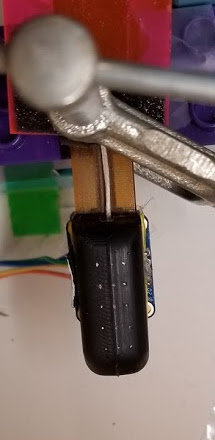
\includegraphics[width=.15\textheight]{images/setup/grid2.jpg}
\caption{Grid of 15 points, marked with silver sharpie applied through holes
poked in a piece of tape.}
\end{figure}

\subsubsection{Instrumentation}
I simply hot-glued an IMU to the underside of the finger. I used was the Bosch BNO055 sensor. A breakout
was available from adafruit.com for \$35, which is relatively inexpensive. I chose this sensor not
only for the built-in processing, and also because of the extensive beginner-friendly documentation
developed by Adafruit for all of its products. It was recommended to me by a
researcher at  
%(person)  at
Right Hand Robotics, which is a spinoff of this lab. I then connected it to an
Arduion Duo, which then relayed the sensor readings over serial to my laptop,
running Ubuntu 16.04.

\begin{figure}[H]
\centering
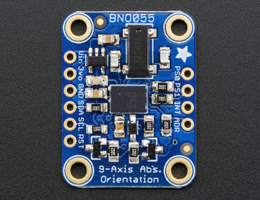
\includegraphics[width=.3\textwidth]{images/setup/bno055.png}
\caption{Adafruit BNO055 9-axis orientation sensor. "Bosch is the first company to get this right by taking a MEMS
    accelerometer, magnetometer and gyroscope and putting them on a single die
    with a high speed ARM Cortex-M0 based processor to digest all the sensor
    data, abstract the sensor fusion and real time requirements away, and spit
    out data you can use in quaternions, Euler angles or vectors." (quote and
    image source: adafruit.com)}
\end{figure}

\begin{figure}[H]
\centering
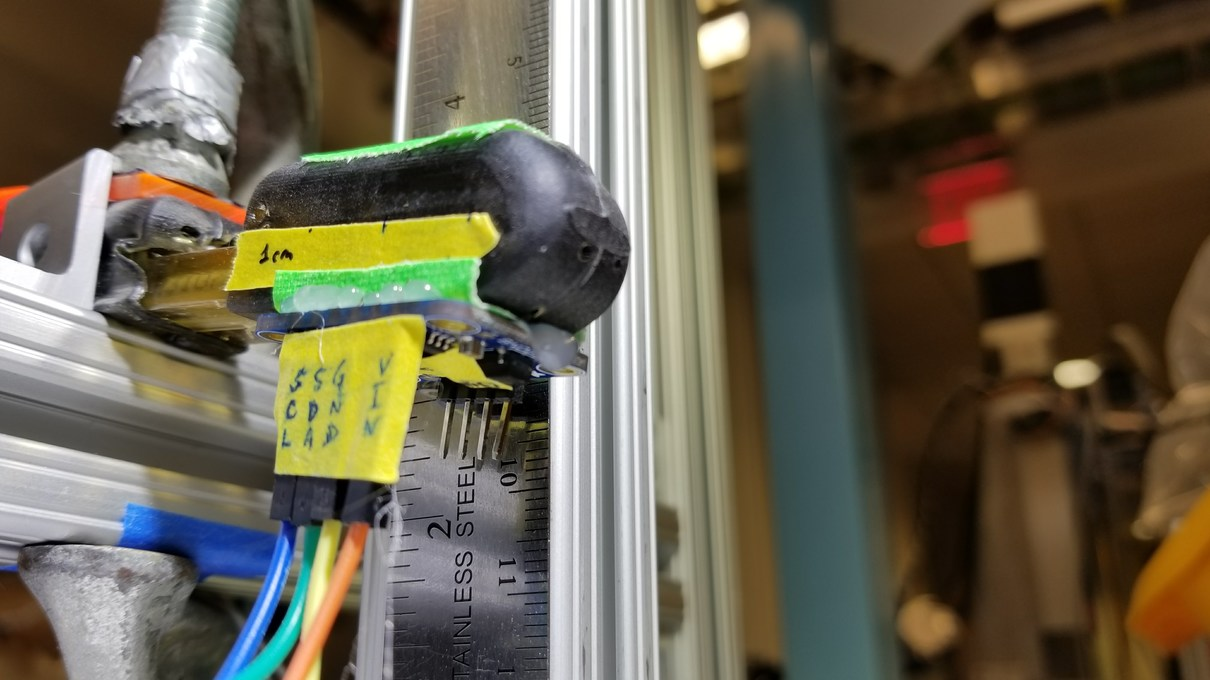
\includegraphics[width=.5\textwidth]{images/setup/IMU.jpg}
\caption{IMU attached to bottom of finger. I made sure that the wires hung
loosely and did not interact with the tabletop and  press up against the finger}
%\label{fig:figura1}
\end{figure}

I also attached an Apriltag (which looks like a QR code) and a Micontracker tag (which has a
checkerboard like cross), both of which can simply be printed out on paper, and calibrated the
webcam for use with the Apriltag C++ script. Although I have collected mictrontracker and apriltag
data for comparing to the IMU deflection data, I have not had a chance to
analyze this data yet.

\begin{figure}[H]
\centering
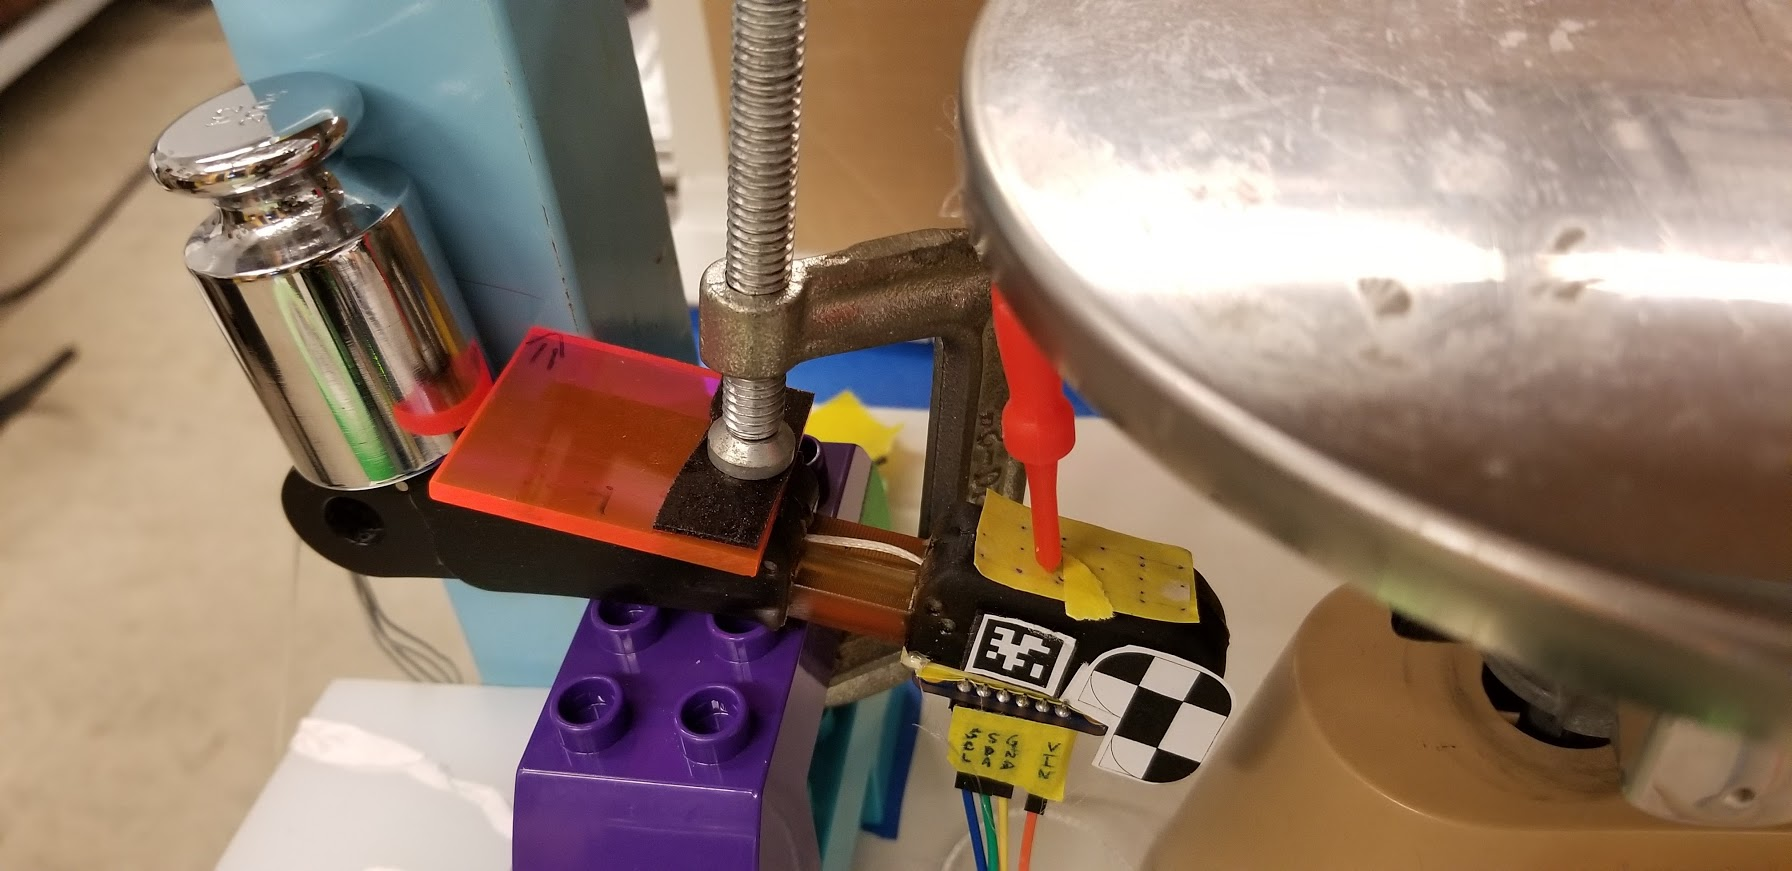
\includegraphics[width=.6\textwidth]{images/setup/microntracker_template.jpg}
\caption{Apriltag on the left and Mictrontracker "Xpoint" on the right}
%\label{fig:figura1}
\end{figure}

Unfortnuately, the IMU acclerometer would consistently refuse to calibrate if the sensor did not
start parallel to the ground. The significant slope of the finger versus the clamp and 90 degree
angle of the 80/20 meant that I had to approximate a slanted 80/20 setup by increasing the degrees
of freedom on the L brackets (removing t-nuts). This led to a lot of worry on my part about the
creakiness and variability in the data collection as I could not guarantee angle consistency,
although in retrospect this is almost completely mitigated by the fact that I am zeroing before
every reading. 


Complications arose from the limited travel of the triple beam balance, which meant I could only
measure small deflections (initially on the order of 4 mm; after discovering that I could take the
end stop off the back edge of the triple beam balance, about 10mm). At the tip of the finger, I
could only less than a hundred grams of "force" (about 1 N), while 4N is a normal amount of force
applied by humans to grasp things. This remained a source of frustration throughout the data
collecting and ate up many hours of adjusting the experimental setup.
Another source of delay was that it took several attempts to find the MiconTracker manual (found on
the old desktop in lab), without which the Microntracker interface was difficult
to use.

In order to apply load to pull on the tendon and change the stiffness of the finger, I decided on a
simple setup where I hung a weight from the tendon.

\begin{figure}[H]
    \centering 
        \subfloat[ Loading the tendon by hanging weights in a paper basket
        ]{%
            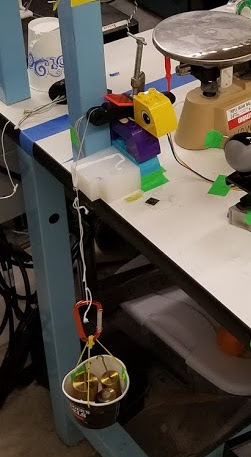
\includegraphics[width=0.28\textwidth]{images/setup/loading.jpg}%
        }\hfil % MUST be right above next figure
        \subfloat[ Loading the end of the finger, to help bring the unloaded
        finger to parallel with the table.
        ]{%
            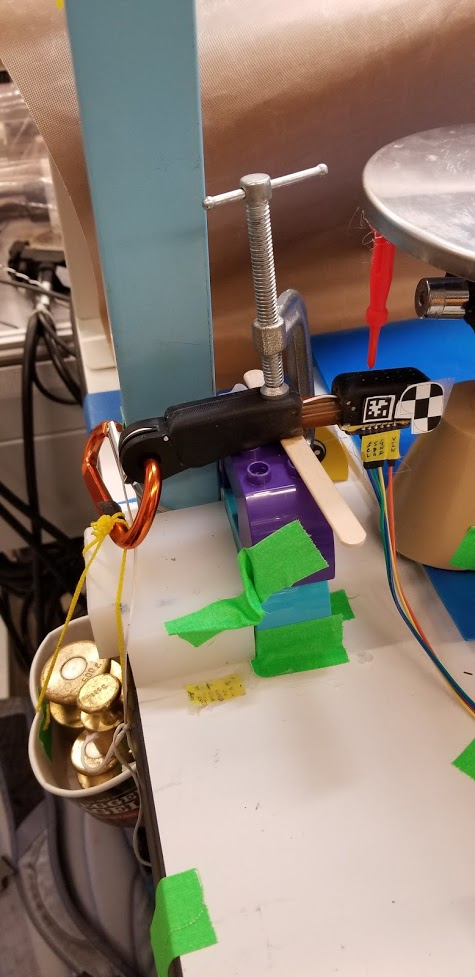
\includegraphics[width=0.25\textwidth]{images/setup/leveling.jpg}%
        }\hfil
        \caption{Experimental setup for collecting data at two different
        stiffnesses (by loading the tendon, as would happen in order for gripper
    to grasp an object)}
\end{figure}


Over time, I trended toward collecting coarser and coarser data as I grew confident
that measurements still provided enough data for me to see overall trends in the data
(such as the linearity of the data). I shifted from 2g increments, to 20g, and in the end 50g
increments. This meant that for the finger when stiffness was applied, I had to change the setup so
that the finger started at an angle and became parallel to the floor when load was applied to the
tendon. After my deep grievances with producing angles on the 80/20 setup, I decided to use legos
with popsicle stick props on one end in order to produce the correct angles.

Finally, I discovered at the very end that I could calibrate the scale to have a constant force
offset. Thus, instead of collecting a zero measurement with the tip starting just above the surface,
which meant that I had to wait for the oscillations to settle, I could put an offset which made the
scale keel all the way to up when the weight was removed. This made zero measurements 2-3x
faster, which reduced the cognitive load to remember which measurement I was at, which both reduced
data cleanup and needing to recollecting data. This led to significant time savings.

\begin{figure}[htbp]
    \centering 
        \subfloat[Scale calibration setup
        ]{%
            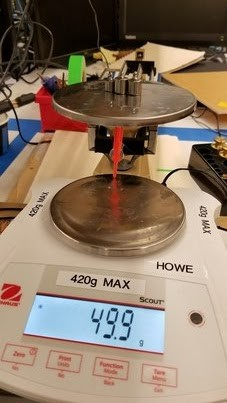
\includegraphics[width=0.2\textwidth]{images/setup/scale_calibration.jpg}%
        }\hfil % MUST be right above next figure
        \subfloat[ Scale calibration graph, with nominal offset of 5g. I observed that the offset is not
constant and increases with increasing load
        ]{%
            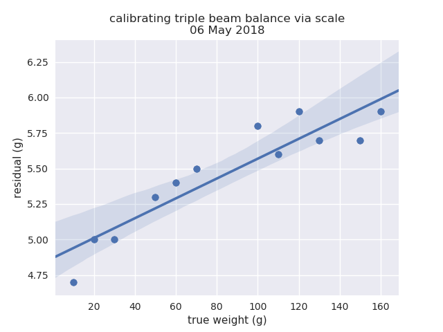
\includegraphics[width=0.5\textwidth]{images/setup/scale_calibration_graph.png}%
        }\hfil
        \caption{Scales and more scales: calibrating the weight applied with the triple beam balance using an electronic scale }
\end{figure}


\section{Data Analysis}

\subsection{Loaded tendon data}

For the final dataset, I aimed to collect data quickly for two different finger tendon loads
(which I'll refer to as relaxed and loaded respectively). I collected data in 50g intervals at two y
locations and three x locations on the finger (total of 6 positions).  Specificially, there were
positions 4,5,6 and 10,11,12.  x = [3.1, 4.1] and y = [0.2, -0.1, -0.4].

(Note that I defined the center line of the finger to be y=0, but as there is a mold line there, the
data is collected from 0.1 mm off of the center line)

First, I conducted a quick sanity check. By plotting torque versus measured theta, I saw that the data follows
a linear pattern, which is what I expected based previous experiments.


\begin{figure}[htbp]
    \centering 
        \subfloat[
        ]{%
            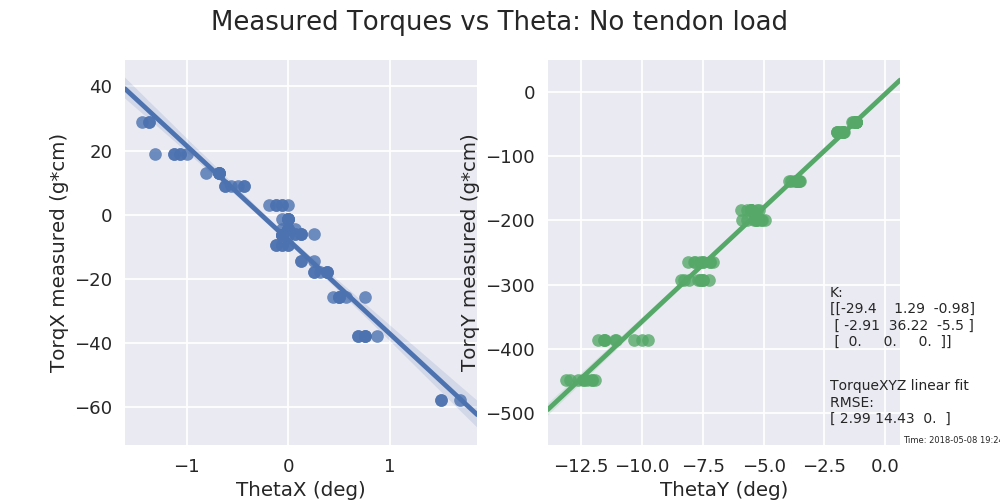
\includegraphics[width=0.9\linewidth]{images/stiff/torqtheta}%
        }\hfil % MUST be right above next figure
        \subfloat[
        ]{%
            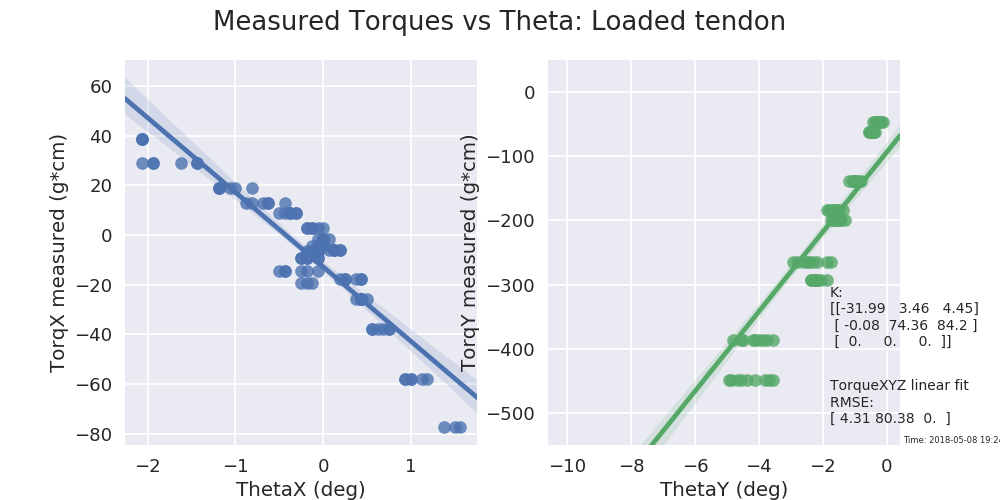
\includegraphics[width=0.9\linewidth]{images/stiff/torqtheta_loaded}%
        }\hfil
        \caption{ Please note that there are two different y labels. The left graph is of Torque X vs Theta X
        (roll), while the right graph is of the Y counterparts (Torque Y vs Theta Y)}
\end{figure}

For the Theta Y (yaw) case, the relaxed tendon fit has a root mean square error (RMSE) of 14.4 (gram
centimeters), or in other words, if the average x position is ~3.5cm, then the average error (for
estimating y-axis torque) is about four grams.

On the other hand, the loaded tendon fit has a much higher RMSE of 80.4 g*cm, which if valid, means
that the average error is about 23 grams. This is a much larger error, and a bit unfortunate given
that we care more about the loaded case in real grasping scenarios. 

I then fit a line to the data, and double-checked my work again. The slope of this line gives us our
stiffness tensor K. I can double check that we've conducted a linear fit by see that we have
by comparing our newly created torque estimates to the
original measurements. The datapoints do not fall precisely on a line because the K matrix and fit
is in three-dimension. In picking a single dimension to plot, the projection results in datapoints
that are not linear in one dimension despite a linear fit overall. The \cref{fig:sanity1} and
\cref{fig:sanity2} reassure me that my code is working. 

\begin{figure}[H]
\centering
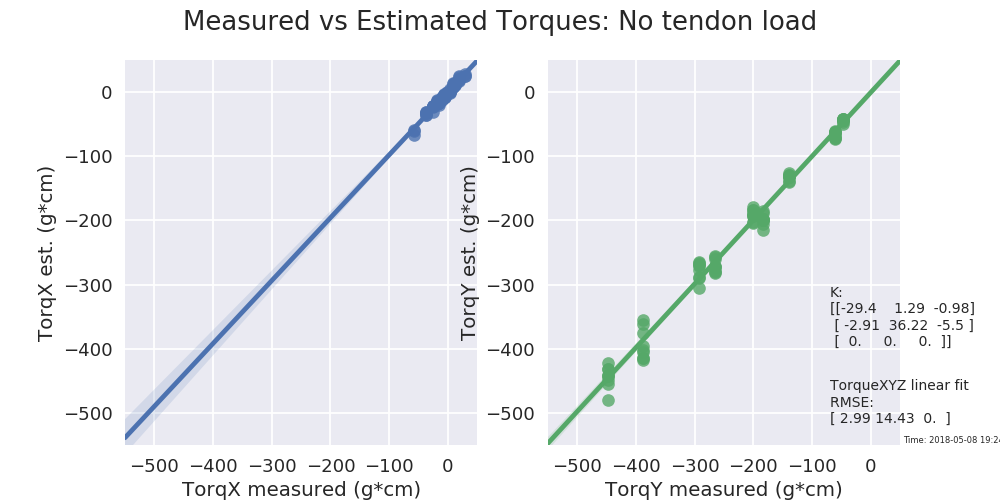
\includegraphics[width=0.9\textwidth]{images/stiff/torqsanity.png}
\caption{Relaxed tendon}
\label{fig:sanity1}
\end{figure}

\begin{figure}[H]
\centering
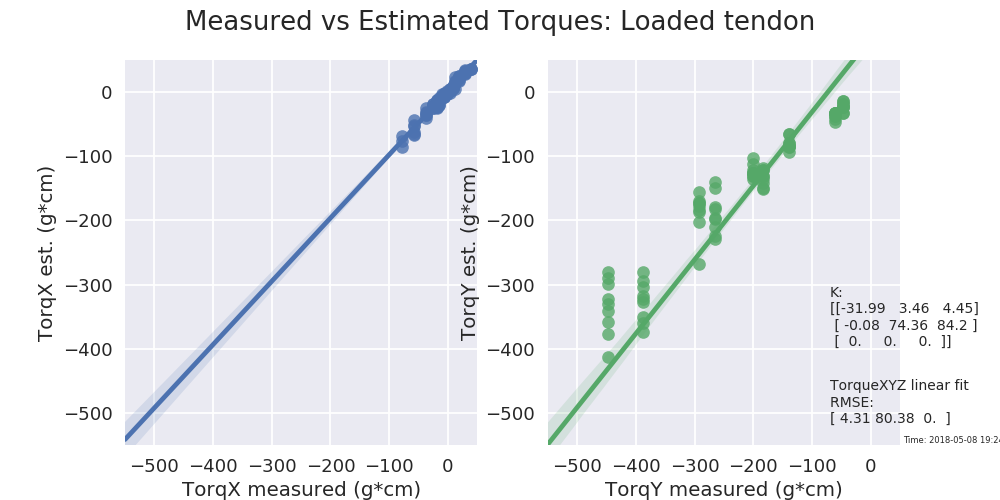
\includegraphics[width=0.9\textwidth]{images/stiff/torqsanity_loaded.png}
\caption{Loaded tendon}
\label{fig:sanity2}
\end{figure}

Next I looked at the residuals. Based on the previous experiment, I was expecting to see a linear
relationship in the residuals between ThetaY and TorqueY. However, I did not see any such
relationship in the relaxed case, which should have most closely matched the data in the previous
experiment (see \cref{init-data}).


However, in \cref{fig:nopattern} there does not appear to be such a pattern, and it seems like the
residuals are somewhat randomly noisy.

\begin{figure}[H]
\centering
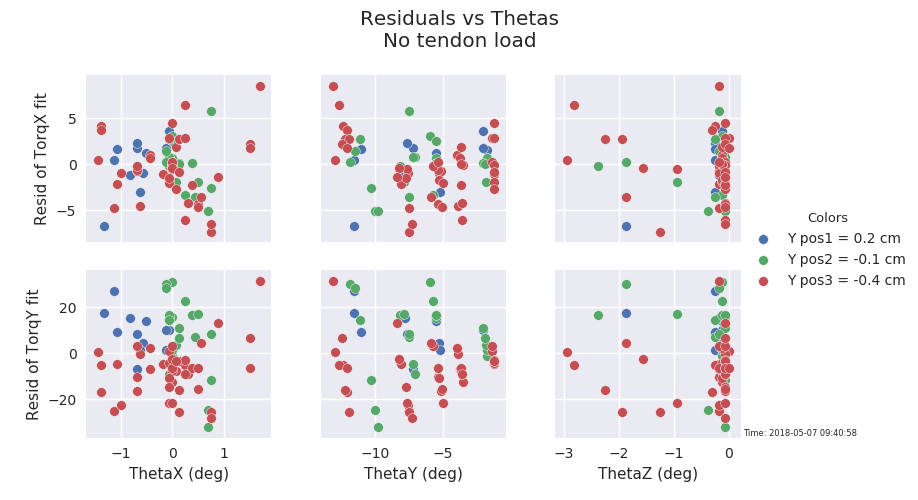
\includegraphics[width=.9\textwidth]{images/stiff/GOODResid_vs_Theta.png}
\caption{Relaxed tendon}
\label{fig:nopattern}
\end{figure}

Confusingly, as shown in \cref{fig:yespattern} a pattern did appear in the loaded case. Note also that the residuals in the loaded case
are much larger. Further investigation will be required to figure out what is going on here.

\begin{figure}[H]
\centering
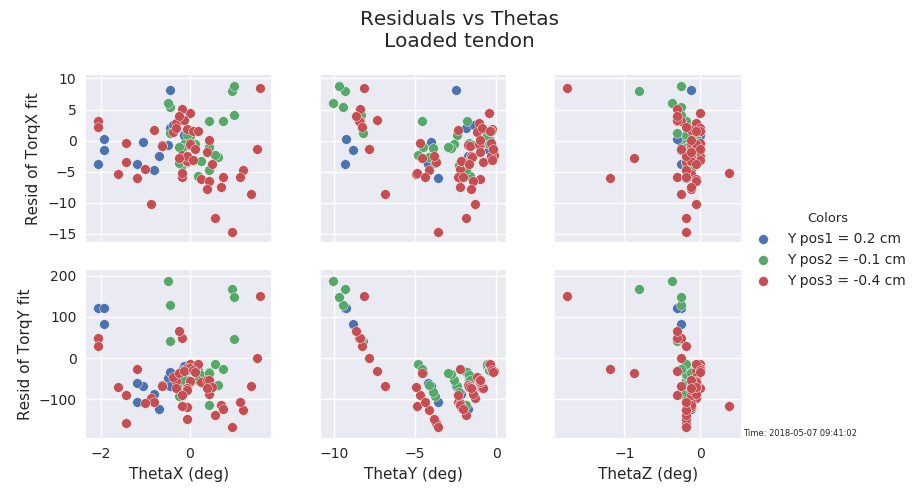
\includegraphics[width=.8\textwidth]{images/stiff/GOODResid_vs_Theta_loaded.png}
\caption{Loaded tendon. NOTE: Patterns in the thetaZ may be ignored as it was not used in the fit,
    due to the assumption that the contact forceZ is always zero.  }
\label{fig:yespattern}
\end{figure}

Perhaps the most satisfying graph that came out of this experiment compares the two stiffness
matrices in the relaxed and loaded cases. See  \cref{fig:comparison}

\begin{figure}[H]
\centering
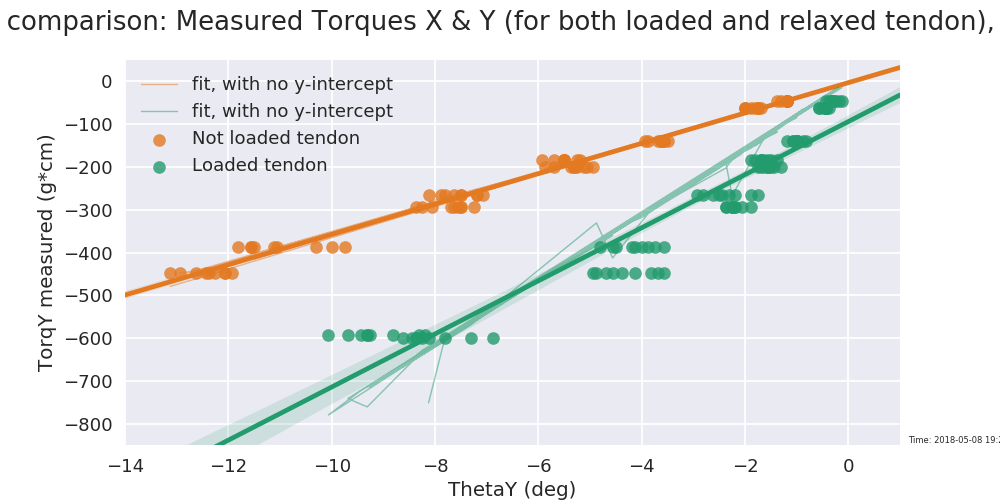
\includegraphics[width=.9\textwidth]{images/stiff/StiffnessComparison.png}
\caption{Loaded case shown in green, relaxed tendon shown in orange. This graph shows that the
loaded tendon is stiffer (slope is steeper), as we expect. Both models seem mostly linear, but it's
possible that in the loaded case, the fit is more exponential. Note that physically the model must
go through the y-intercept, and I have graphed the actual fit used to calculated residuals in light
green (albeit for a nonlinear fit). The dark green line is plotted only due to limitations in my plotting
library.}
\label{fig:comparison}
\end{figure}

\subsection{Initial Experiment: 15 positions, with the relaxed tendon only}
\label{init-data}

The experiment directly prior to the final experiment consisted of collecting nearly 500 points,
mostly in 20g increments, from all 15 positions labelled on the finger (albeit a different finger,
which did not have a tendon string in it -- I had to change fingers because of that).

I started with a sanity check as before, and plotted the estimated vs measured torques.

\begin{figure}[H]
    \centering 
        \subfloat[
        ]{%
            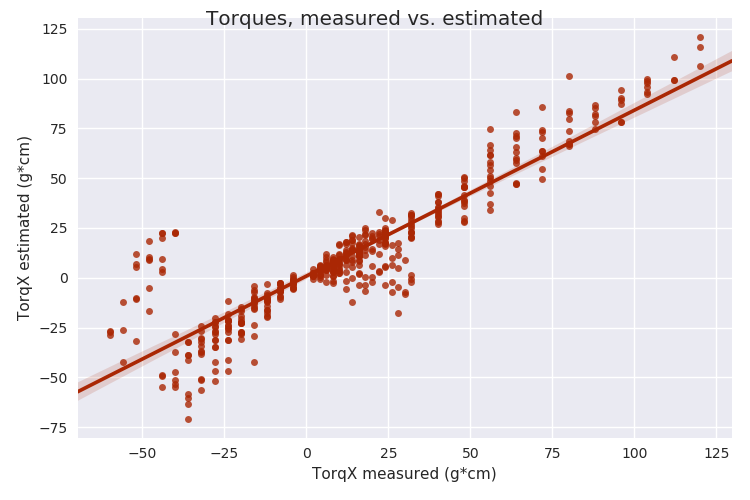
\includegraphics[width=0.48\textwidth]{images/round1/Nocolor_torqX.png}%
        }\hfil % MUST be right above next figure
        \subfloat[
        ]{%
            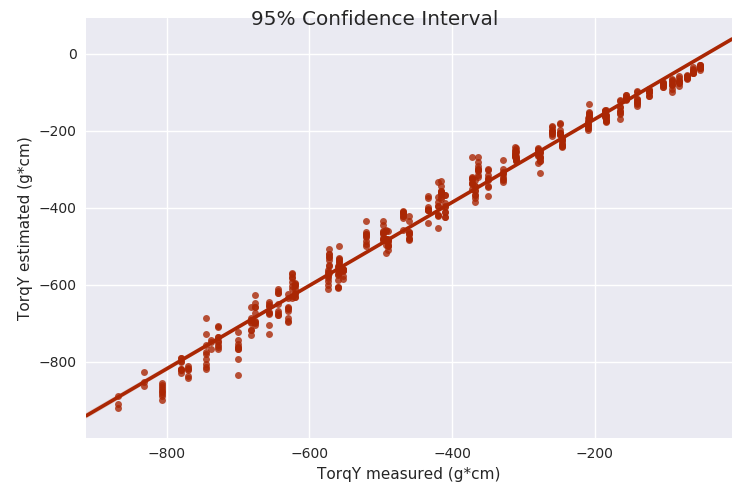
\includegraphics[width=0.48\textwidth]{images/round1/Nocolor_torqY.png}%
        }\hfil
        \caption{Measured torques on the X axis, and estimated torques on the Y axis.
            The left graph shows the X axis (roll) measurements, note the magnitude is much smaller
        compared to the Y axis torque (yaw) measurements. Please ignore the erroneous title on right graph.}
\end{figure}


%\begin{figure}[H]
%\centering
%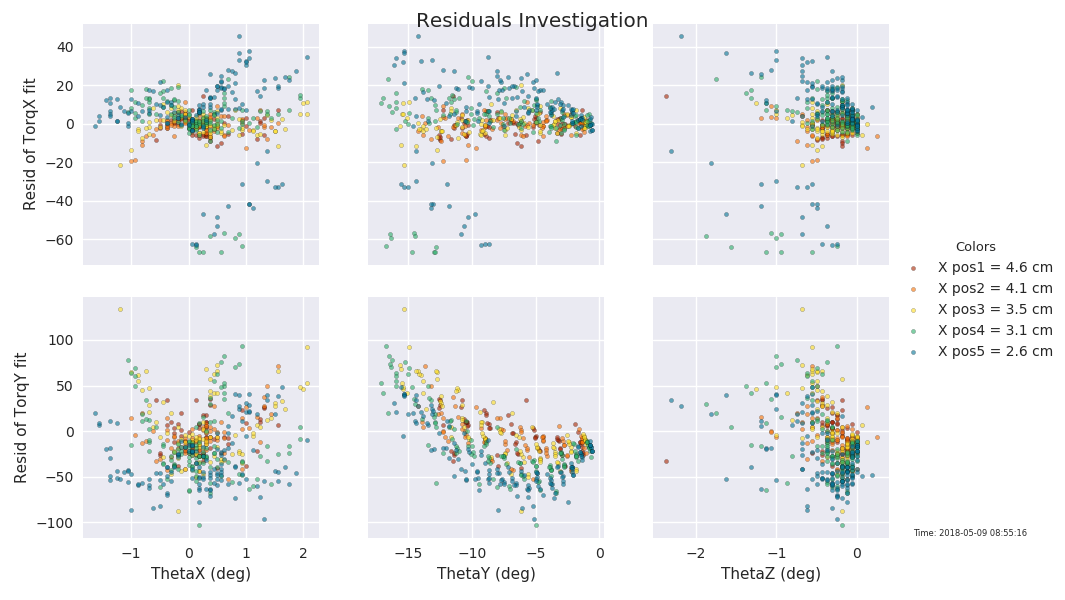
\includegraphics[width=1\textwidth]{images/round1/resids_Theta_coloredX.png}
%%\caption{Loaded tendon}
%%\label{fig:figura1}
%\end{figure}
The large residuals on the left were alarming. To take a closer look at what was going on, I colored
the graph in by X and by Y positions. In \cref{fig:x} we see that all of the datapoints way off the
line come from xpos4 and xpos5, specifically from y = -0.2cm (from  \cref{fig:y}). This does not
seem to be a fluke, as these are not sequential measurements (positions 12 and 15 respectively).

%\begin{figure}[H]
    %\centering 
        %\subfloat[
        %]{%
            %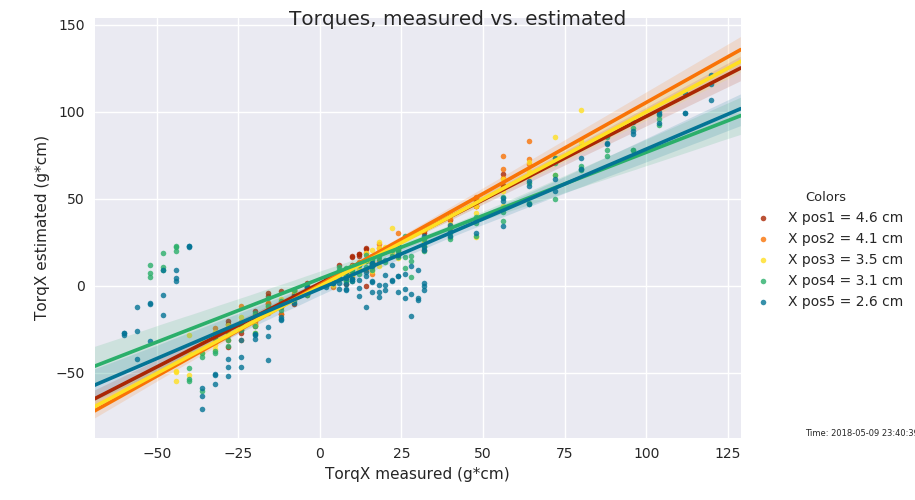
\includegraphics[width=0.5\textwidth]{images/round1/TorqX_Colors_X.png}%
        %}\hfil % MUST be right above next figure
        %\subfloat[
        %]{%
            %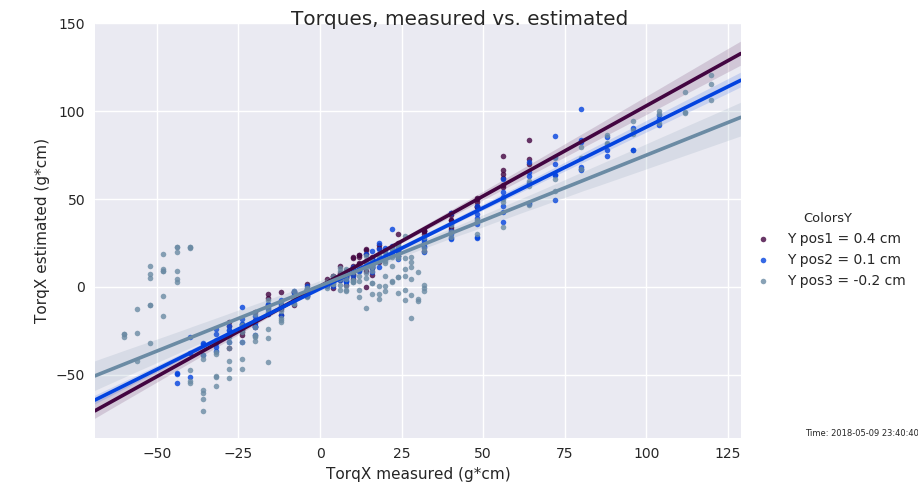
\includegraphics[width=0.5\textwidth]{images/round1/TorqX_Colors_Y.png}%
        %}\hfil
        %\caption{Measured torques on the X axis, and estimated torques on the Y axis.
            %The left graph shows the X axis (roll) measurements, note the magnitude is much smaller
        %compared to the Y axis torque (yaw) measurements. Please ignore the erroneous title on right graph.}
%\end{figure}
\begin{figure}[H]
\centering
            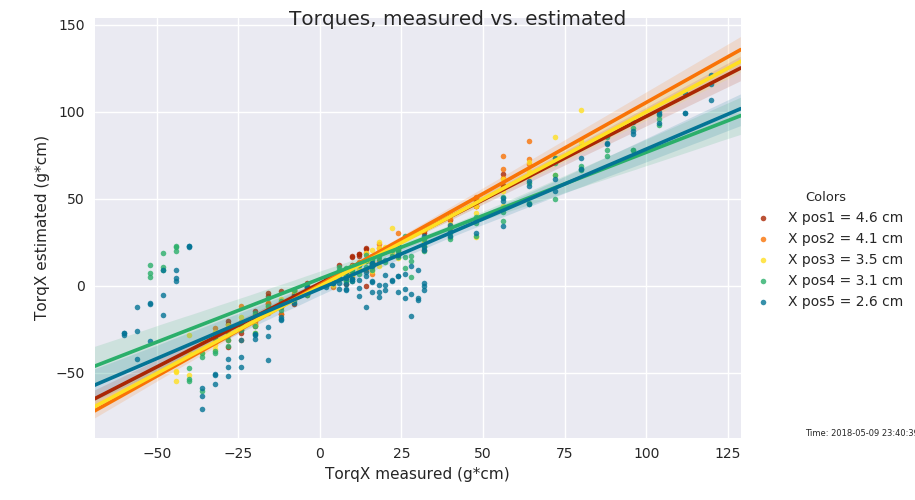
\includegraphics[width=0.9\textwidth]{images/round1/TorqX_Colors_X.png}%
            \caption{Torque measured vs estimated, colored in by X position}
\label{fig:x}
\end{figure}

\begin{figure}[H]
\centering
            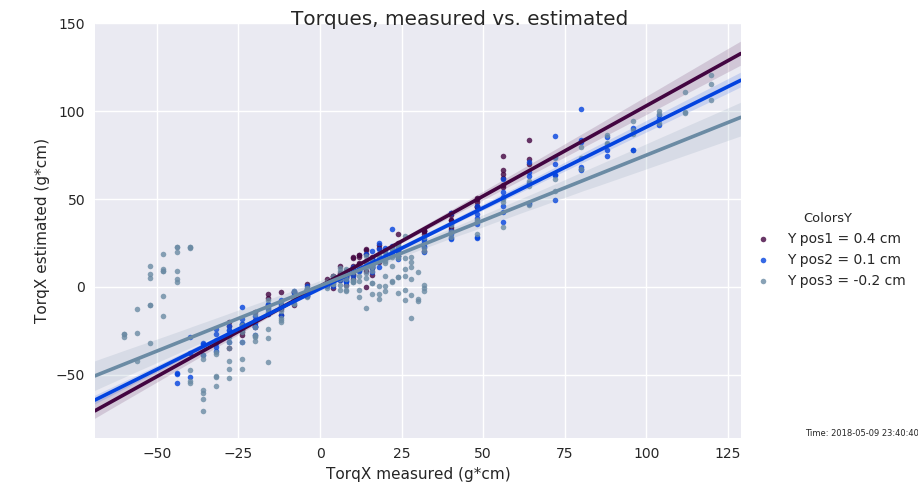
\includegraphics[width=0.9\textwidth]{images/round1/TorqX_Colors_Y.png}%
\caption{Torque measured vs estimated, colored in by Y position}
\label{fig:y}
\end{figure}


\begin{figure}[H]
\centering
            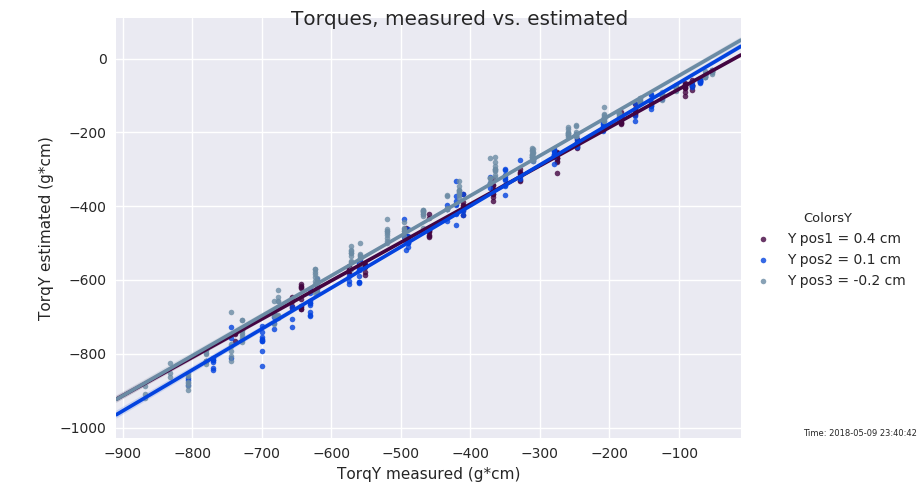
\includegraphics[width=0.9\textwidth]{images/round1/TorqY_Colors_Y.png}%
            \caption{By comparison, the torque Y fit seems very clean.}
\end{figure} 
%(For the same graph colored
                %in by X position, see \cref{fig:yX}

I then systematically plotted the residuals against the factors that might 
affect them: the torques, forces, and angular deflection amounts. For instance, it seems plausible
that, as the amount of force applied increases, the residuals might increase.


\begin{figure}[H]
\centering
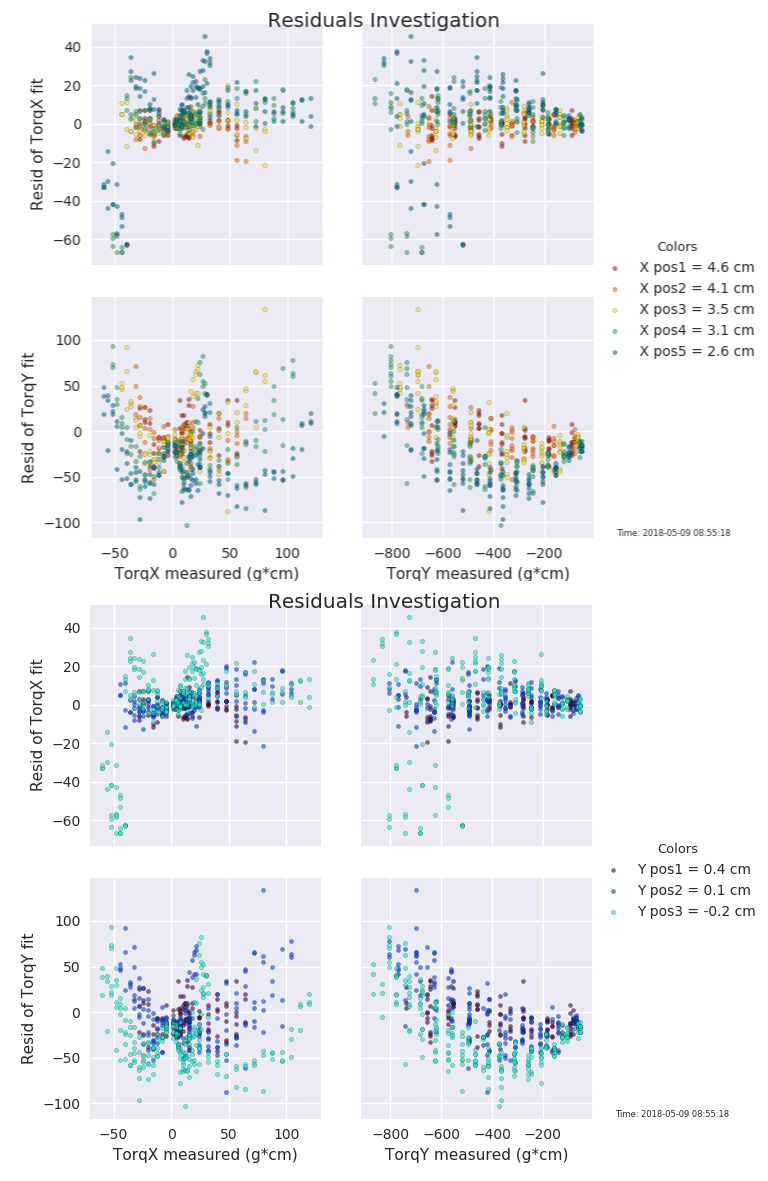
\includegraphics[width=.95\textwidth]{images/round1/resids_Torq.png}
\caption{Torque estimate residuals versus torques estimates, colored by their X or Y positions.
There does appear to be a suspicious trend between the residuals and the torque Y measurement.}
%\label{fig:figura1}
\end{figure}

%\begin{figure}[H]
%\centering
%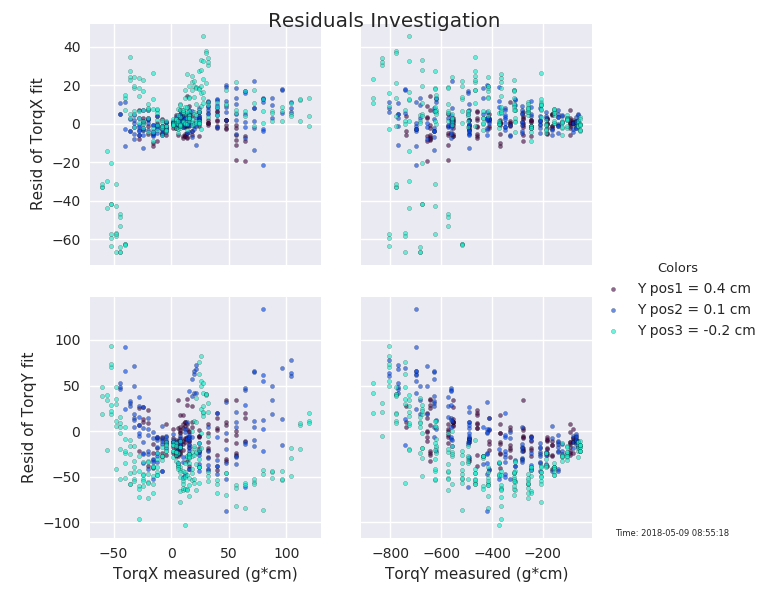
\includegraphics[width=.9\textwidth]{images/round1/resids_Torq_coloredY.png}
%%\caption{Loaded tendon}
%%\label{fig:figura1}
%\end{figure}

\begin{figure}[H]
\centering
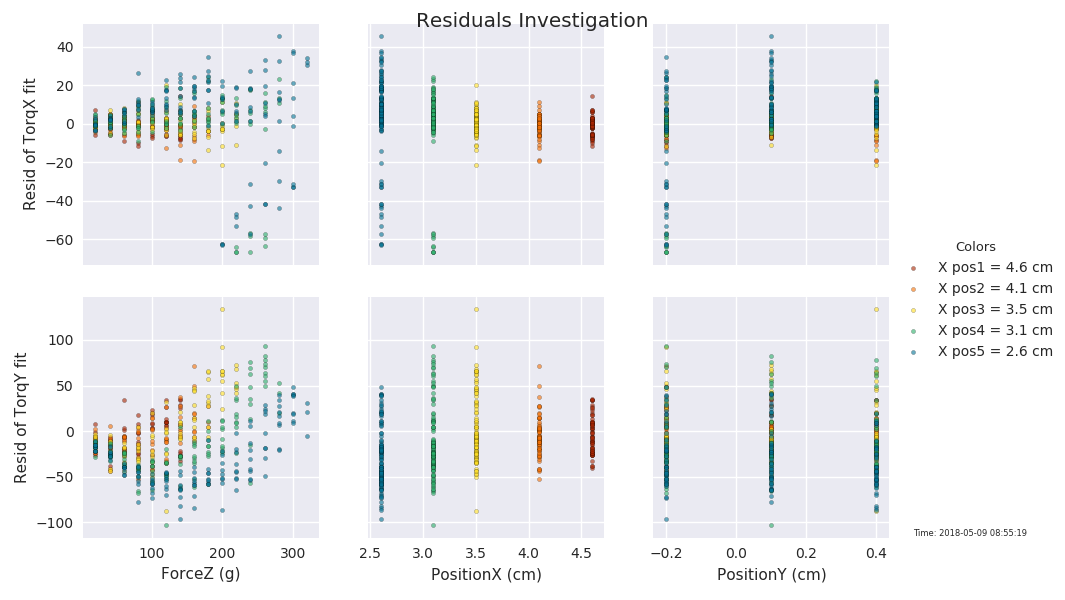
\includegraphics[width=1\textwidth]{images/round1/resids_Force_coloredX.png}
\caption{There seems to be generally somewhat random residuals, except there's a chunk of large
residuals on the upper right graph of TorqX residuals vs force applied. I never resolved the cause
of this. Additionally, note that the first X position, where the finger is least stiff, has a
noticeably different set of residuals than the other positions.}
%\label{fig:figura1}
\end{figure}

For additional graphs, please see \ref{appendix-graphs}.
%\begin{figure}[H]
%\centering
%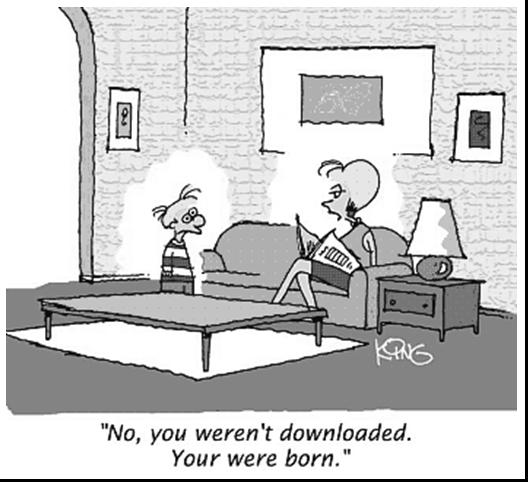
\includegraphics[width=.3\textwidth]{fig1.jpg}
%\caption{Exemplo de figura}
%\label{fig:figura1}
%\end{figure}
\section{Attempted fit improvements}
\subsection{Experiment: 15 positions, relaxed tendon only}

K estimate, bylinear regression (no y intercept)
Torque = K * Theta
Residual
RMSE Lin K, no resid: 36.63
Residual prediction using Theta
Corrected Torque Estimate
RMSE Lin K, Lin resid 26.65
RMSE Lin K, RF resid 22.56

Finally, I briefly attempted to do the "use machine learning or other methods to fit the residuals
and improve the overall torque estimate". 

\begin{table}[H]
    \centering
    \caption{Comparison of fits}\label{tab:MDP_calibration}
    \begin{tabular}{l|c|c|c|c|c|c}
         \hline \hline
         &  Linear & Polynomial & Gradient Boost & Adaboost & Random Forest\\
         \hline 
         Black Box          & 36.1 & 9.2 & 15.8 & 25.1 & 80.4 \\ 
         Corrected Linear fit & 28.5 & 18.8 & 18.8 & 25.1 & 52.9 \\
    \hline
    \end{tabular}
\end{table}


\begin{table}[H]
    \centering
    \caption{Brief investigation of fitting residuals on relaxed+loaded experiment}\label{tab:MDP_calibration}
    \begin{tabular}{l|c|c|c|c|c|c}
         \hline \hline
         &  Linear & Polynomial & Gradient Boost & Adaboost & Random Forest\\
         \hline 
         Black Box          & 36.1 & 9.2 & 15.8 & 25.1 & 80.4 \\ 
         Corrected Linear fit & 28.5 & 18.8 & 18.8 & 25.1 & 52.9 \\
    \hline
    \end{tabular}
\end{table}


\begin{figure}[H]
\centering
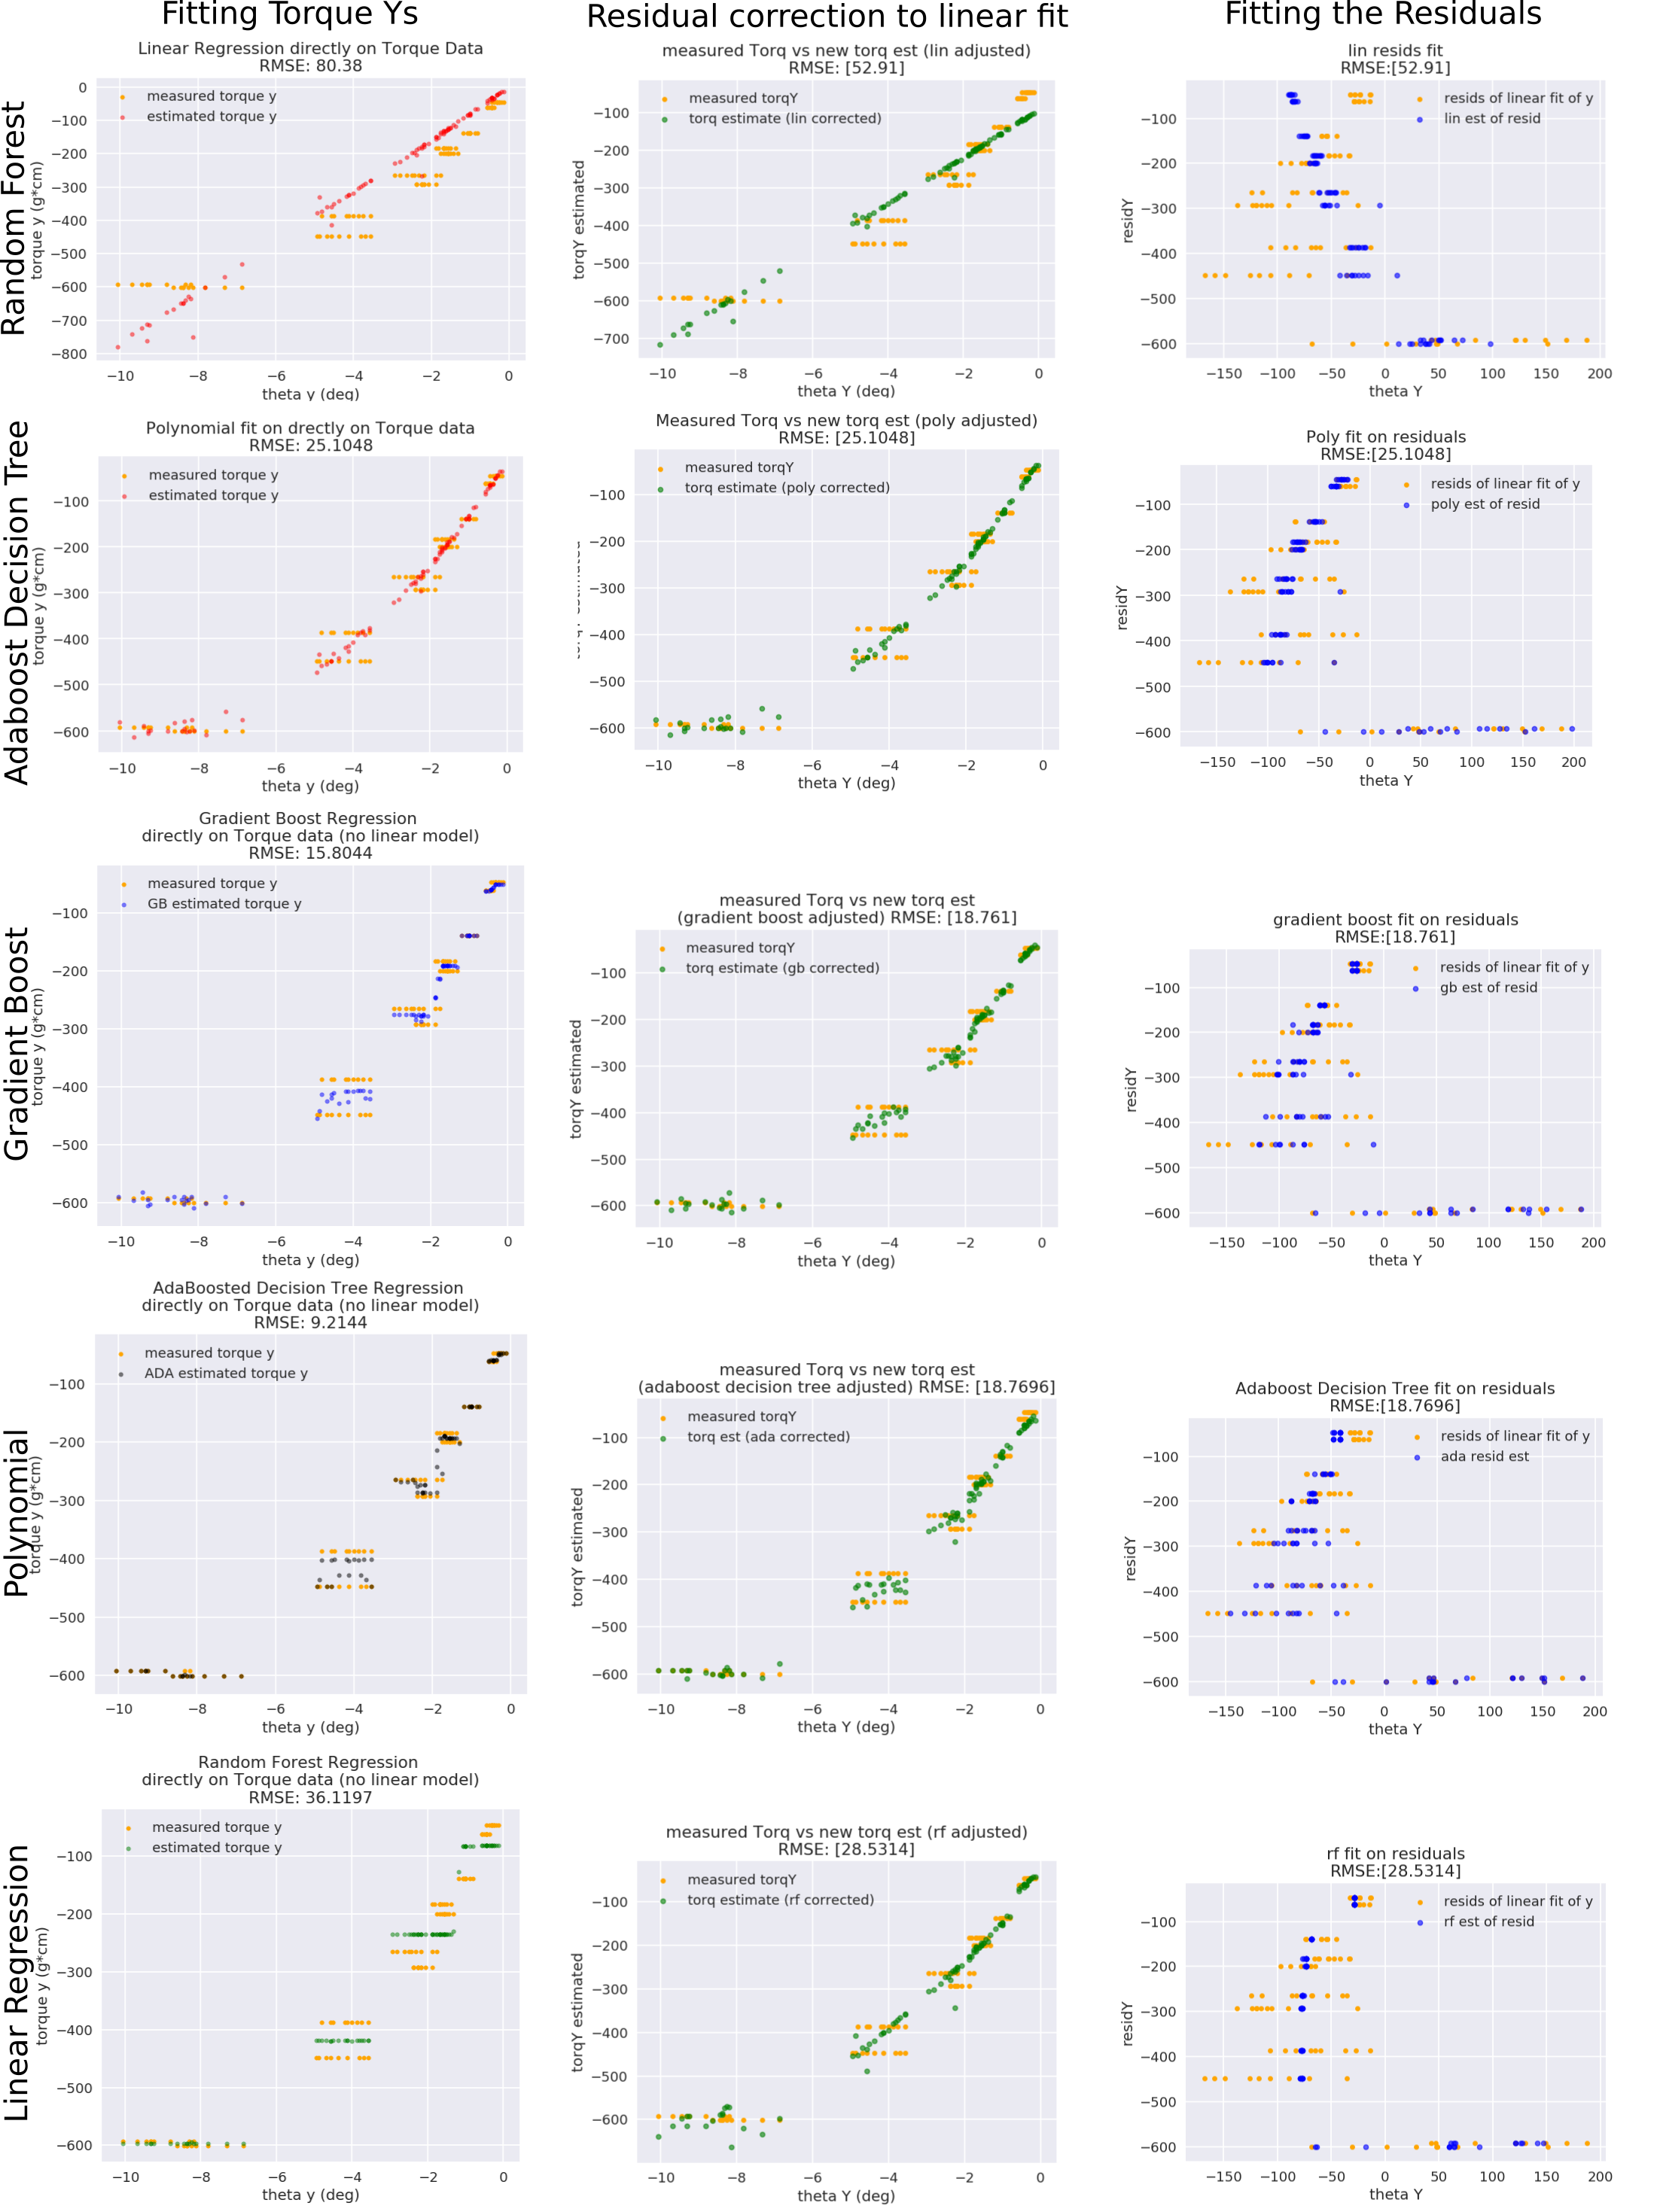
\includegraphics[width=\textwidth]{images/residcorrect/layout_vertical.png}
\caption{How much does it improve our torque predictions to include an estimate of the residuals on
our linear physical model?}
%\label{fig:figura1}
\end{figure}

\section{Sensor Design}

For datasheets, please see \ref{appendix-sensors}.

\begin{figure}[htbp]
    \centering 
        \subfloat[ a caption
        ]{%
            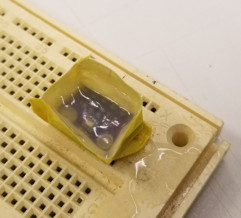
\includegraphics[width=0.2\linewidth]{images/sensor/sensor.jpg}%
        }\hfil % MUST be right above next figure
        \subfloat[ caption b
        ]{%
            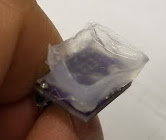
\includegraphics[width=0.2\linewidth]{images/sensor/sensor2.jpg}%
        }\hfil
        \subfloat[ caption c
        ]{%
            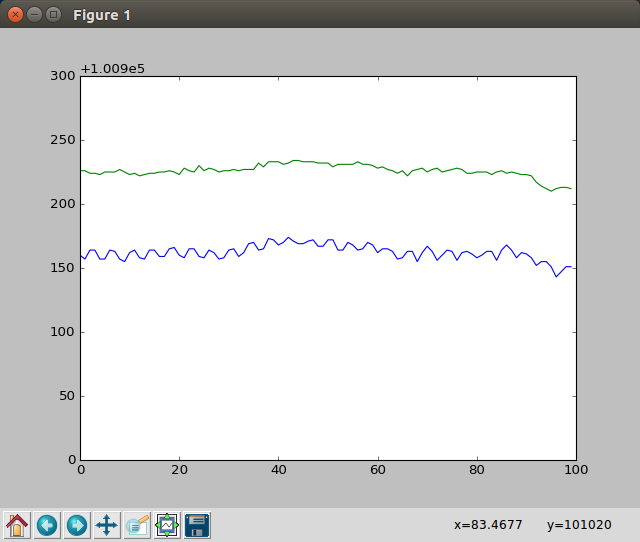
\includegraphics[width=0.5\textwidth]{images/sensor/analog_plot.png}%
            \label{fig:c}%
        }\hfil 
    \caption{ Overall caption.}
\end{figure}

I produced Arduino and python code that allowed me to view a plot in real time of the sensor data.

I also integrated the Arduino with an RGB LED strip, where if you pressed on the sensor,
more LEDs would light up.

\begin{figure}[H]
\centering
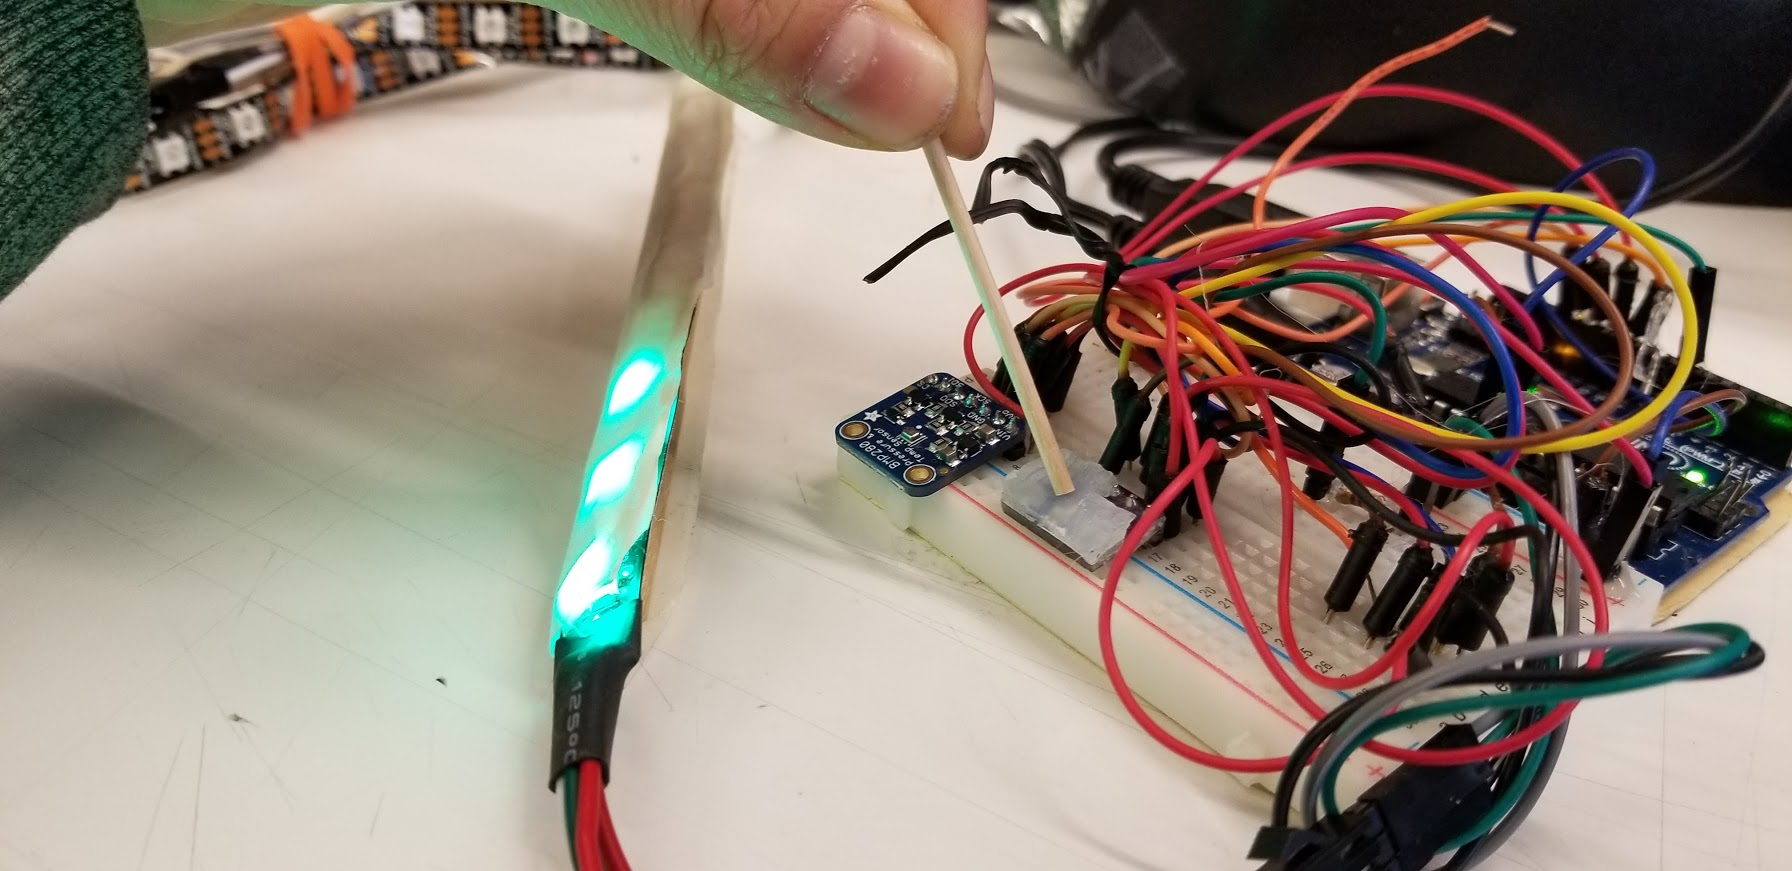
\includegraphics[width=.8\textwidth]{images/sensor/poke.jpg}
\caption{LED setup. The left (blue) PCB is an Adafruit breakout available for
\$10. The generic breakout can be had for less than a \$1 (it has fewer
components, e.g. does not support 5V input}
%\label{fig:figura1}
\end{figure}

The sensor showed a large amount of hysteresis, which should be investigated and addressed.

Note that the setup required use of a separate power supply, otherwise the Arduino would refuse to talk to the
computer (for real-time plotting) when the LED strip drew load on the 5V line.

Evaluation of the sensor is ongoing. It has a built-in pressure sensor, which
can be used to compensate for temperature changes (for instance, if you press on
it with your finger, the heat compounds the reading and also resuls in a
noticeably tail as the heat dissipates relatively slowly.

\section{Knowledge}

In the process of this research, I learned about how accelerometers are calibrated, which I found
very interesting (although ultimately, thanks to the built-in sensor fusion and calibration routines of the BNO055
sensor, I did not need to write my own calibration routines). The common presence of the gravity
vector across meaurements at diffent angles makes this calibration possible.

I learned the most about exploratory statistical data analysis. Where previously I had not even
heard of residuals (only scalar measurements such as mean-square-error), I learned about how they
could be compared to a horizontal basis against which they would be randomly distributed assuming
random noise around a proper physical model.

Finally, I learned more about the I2C and SPI protocols for receiving (and writing) to multiple
sensors. I began work on creating a custom printed circuit board to create a 3x4 array of sensors,
and decided to switch and learn to use a newcomer in the PCB design space, which has CERN support: the free and open-source
KiCAD tool.

\section{Conclusions}

The stiffness of the finger was remarkably linear, which meant that machine learning and higher
order terms had little to contribute to improving the fit between measure theta deflections and
force estimates. Thus, the IMU appears to have much to contribute to estimating forces applied to
the finger. However, caution is necessary, since in actual grasping, as Qian demonstrated, the
axis I measured becomes the stiffest axis when the tendon is pulled taut to grasp an object.It bends
relatively little compared to the other axes.

%However, I was only able to apply relatively small loads to the finger. It's possible that with
%large loads, the stiffness becomes less linear, in which case linear fit residuals may become more
%prominent or structured. If this were the case, machine learning approaches might have more to
%contribute to the force estimates. As it were, the data I collected did not benefit much from the
%addition of non-linear models fitted with machine learning techniques such as random forests.

%Most crucially, Qian demonstrated to me the process by which grasps fail. By observing the grasping,
%I discovered that when the tendon was pulled taught (as needed to grasp anything), the y-axis was now
%now the stiffest axis! Thus, characterizing the finger with no tendon load applied and primarily in
%the y-axis direction, while a great learning experience, does not generalize at all to practice and becomes a
%toy example.

Qian also showed me how the finger relied extensively on mechanical mechanism intelligence (as opposed to full
actuated parallel grippers, commonly used in computer science labs). I saw that complete failures
tended to occur because the finger had failed to detect contact when contact had already occured.
This suggests the better instrumentation of the finger is critical. The IMU by itself can only
suggest contact force, and the tactile sensors are needed to tell contact location. To evaluate the
contribution of the IMU to force estimates and not just torque estimates, we must build better
location sensors than the current 1x4 array.

%Referências bibliográficas devem ser utilizadas dentro de um estilo uniforme e não ambíguo. A SBC sugere os seguintes formatos para referências: \cite{knuth:84}, \cite{boulic:91}, e \cite{smith:99}.

%\bibliographystyle{sbc}
%\bibliography{sbc-template}

\subsection{Future Work}

The microntracker should be used to evaluate the IMU. Evaluating the use of Apriltags with the
microntracker would help reproducibility by others (or future grad students), as webcams are cheap
and readily available, and documentation for apriltags is freely available online.

A full sensor array on a custom PCB, manufactured into a finger unit, should be
developed and characterized. By collecting data and then fusing this with the IMU data, we could
physically evaluate the grasp stability preductions, producing an important tie between theory and
practice to ensure the two complement each other. The important of this has been mentioned above.

\section{Thanks}

Thanks To Qian, who took a lot of time out of her busy about-to-graduate life to explain her
research and the field of grasping to me. Thanks to Buse, who I really enjoyed talking to and look
forward to getting to know more over the years. Thanks to Alperen for patiently explaining
Micontrackers and training me in lab safety, Yash for some terrible jokes and stepping in when I
needed to push back my final presentation, James Weaver for very late night encouragements, and to
my friends at MD309 and my fellow first-year SEAS PhD students.  And thanks to Prof. Robert Howe for 
patiently giving me a fairly gentle introduction to the world of research, and offering to advise
me.

\section{Felicitous news}

Semester is over! The future awaits, and it seems likely to be full of robots.

\newpage

\clearpage
\vspace*{\fill}
\begin{center}
\begin{minipage}{.6\textwidth}
\Huge
\centering{Appendix}
\normalsize
\end{minipage}
\end{center}
\vfill % equivalent to \vspace{\fill}
\clearpage

\appendix

\section{Apriltags}
I decided to investigate apriltags, which helped me refresh on my knowledge of C++. I struggled to
find an appropriate ROS driver, and ultimately was able to get the C++ working (despite some issues
with the openCV version on my laptop) with the help of Patrick from Prof. Kuindersma's lab.

Example data output
\begin{ttlisting}
2 tags detected: 
Id: 1 (Hamming: 0) distance=0.079741m, x=0.000532, y=0.006102, z=-1.487915, yaw=-0.134615, pitch=0.071828, roll=-0.041146
Id: 7 (Hamming: 0) distance=0.079741m, x=0.000532, y=0.006102, z=-1.487915, yaw=-0.134615, pitch=0.071828, roll=-0.041146
14.9312 fps
\end{ttlisting}

My issues with the openCV version were simply solved by specifiying the openCV
version the compiler should use, as I had two versions on my laptop.

\begin{ttlisting}
nrw@earlgrey:~/projects/apriltags$ vi CMakeLists.txt 
    (line 14) find_package(OpenCV 2.4.9.1 EXACT REQUIRED)
\end{ttlisting}

\begin{figure}[H]
\centering
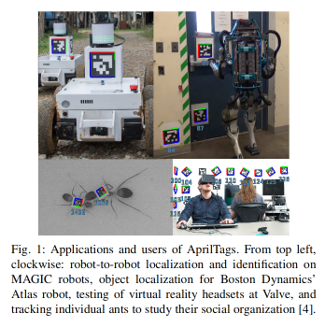
\includegraphics[width=.4\textwidth]{images/april/applications_april.png}
\caption{Applications of apriltags. Figure from: Wang, John, and Edwin Olson. "AprilTag 2: Efficient and robust fiducial detection." IROS 2016.}
%\label{fig:figura1}
\end{figure}

To calibrate the camera, I was able to find a (very!) well-documented python script online that allowed be to calibrate the camera simply by taking a few pictures of a checkerboard.

\begin{ttlisting}[language=C++,breaklines]
(venv) nrw@earlgrey:~/projects/video2calibration$ ./calibrate.py example_input/chessboard.avi calibration.yaml --debug-dir out
\end{ttlisting}

\begin{figure}[H]
\centering
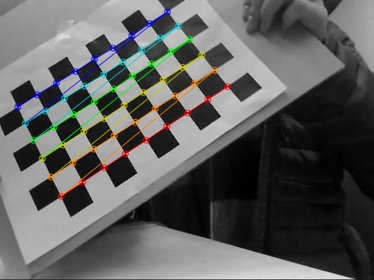
\includegraphics[width=.4\textwidth]{images/april/webcam_calibration.png}
%\caption{Loaded tendon}
%\label{fig:figura1}
\end{figure}

Using the output of the calibration script, I could then set the values in the apriltag example code
to give me (fairly accurate) estimates of the xyz location of the finger in real-world units.

\begin{ttlisting}[language=C++,breaklines]
nrw@earlgrey:~/projects/video2calibration$ ./calibrate.py ~/Videos/Webcam/2018-03-26-112657.webm calibration.yaml --debug-dir out

Performing calibration...
 RMS: 0.442700776066
 camera matrix:
 [[ 666.78668352    0.          343.73827809]
 [   0.          665.79103853  227.19081685]
 [   0.            0.            1.        ]]
 distortion coefficients:  [  6.06301194e-02  -1.94620209e-02   1.45555284e-04   1.24410189e-03
 -2.51439333e-01]
\end{ttlisting}

I did not use the distortion coefficients in the apriltags measurements. These
coefficients, I believe, correct for fisheye and higher order distortions in the
camera images.

\begin{lstlisting}[language=C++,breaklines]
public:

  // default constructor
  Demo() :
    // default settiwgs, most can be modified through command line options (see below)
 [...excerpted section...]
    m_width(640),
    m_height(480),
    m_tagSize(0.00944), // in meters
    m_fx(667), // in pixels
    m_fy(666), //
    m_px(344), // principal point
    m_py(227),
\end{lstlisting}


\newpage

\section{Project Management}

In order to improve time estimates in the future, I find it helpful to look back
at the original timeline. 

\begin{figure}[H]
\centering

\includegraphics[width=.9\textwidth]{images/misc/timeline.png}
%\caption{Loaded tendon}
%\label{fig:figura1}
\end{figure}

From this chart, we can see that I wasn't able to get much traction on my
milestones the first month. Then I spent half a month figuring
out how to set up and analyze an experiment (for instance, understanding how to
analyze data and plot residuals, as well as the point of fitting residuals). Finally, I performed an
abbreviated version of the first 6 weeks squeezed into the last six weeks, and
turned in the last two milestones a week+ late.

Although this seems like a dire in terms of project management, I did  spend a
lot of time on items related to research but not listed directly as milestones. 
I spent a lot of time learning about the grasping field. Additionally designing and
prototyping a new sensor was not on the milestones. As a result, by taking a longer-term view, I
personally do not feel as disappointed as I might be, given my personal goals such as making progess
toward understanding the research process and learning concrete skills.

\section{Outside Resources}

Here is a well-formatted version on Wikipedia describing the 3D stiffness tensor. 

\begin{figure}[H]
\centering
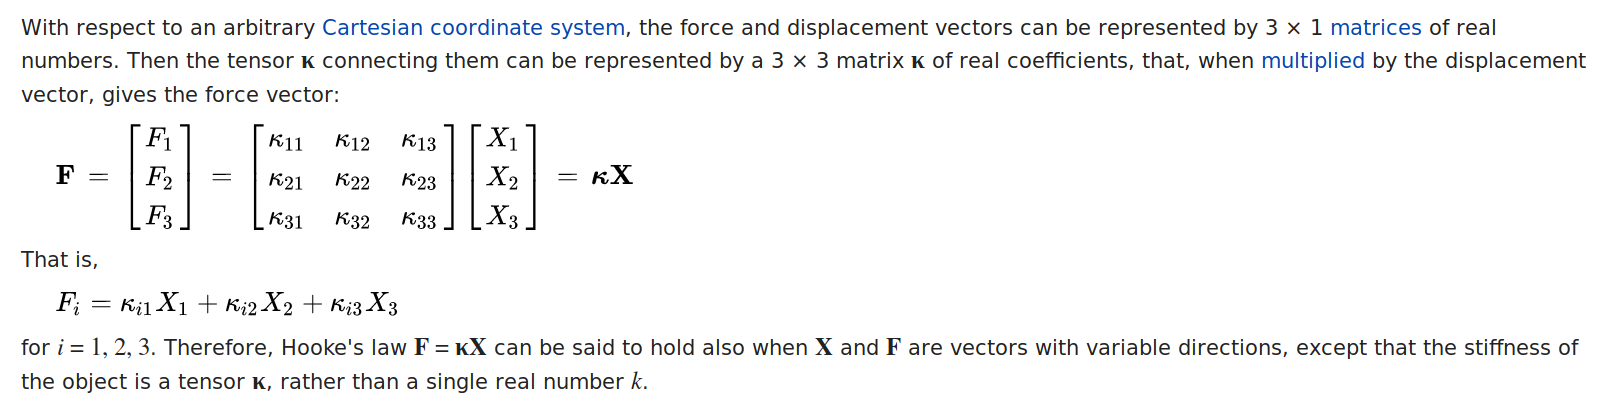
\includegraphics[width=\textwidth]{images/misc/stiffness_tensor.png}
%\caption{Loaded tendon}
%\label{fig:figura1}
\end{figure}



\newpage

\section{Hexo: Online documentation}

I documented my work on a blog, \url{http://orangenarwhals.github.io/}, using the Hexo flatfile content
management system. I chose this because it allowed me to host for free on github, allowed for easy
version control of content, and also had an admin plugin that allowed me to drag-and-drop images,
which is crucial for documenting experiments where I have a lot of graphs. I was also able to get
Latex to work on the site so that I could have equations rendered on there.

\begin{figure}[H]
\centering
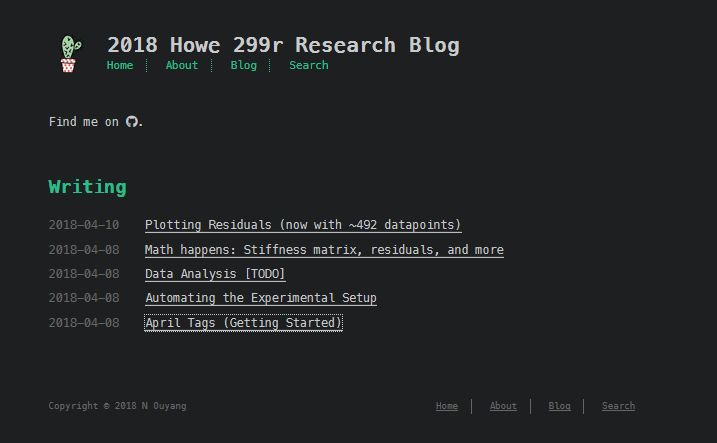
\includegraphics[width=0.8\textwidth]{images/misc/blog.png}
%\caption{Loaded tendon}
%\label{fig:figura1}
\end{figure}


\begin{figure}[H]
\centering
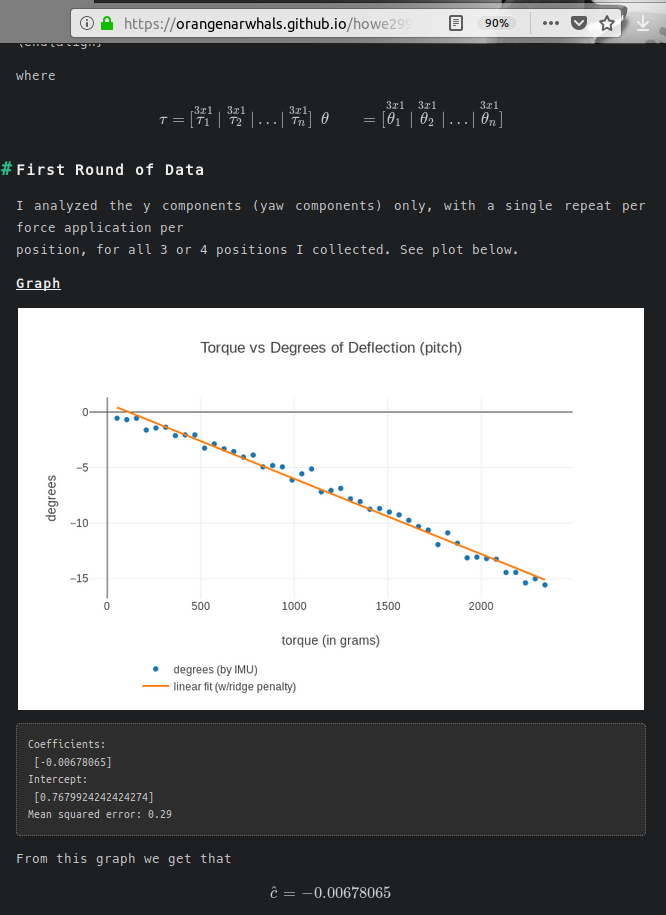
\includegraphics[width=0.8\textwidth]{images/misc/blog_latex.png}
\caption{Getting MathJax (a javascript in-browser version that renders Latex
equations in your webpages) to work was a major source of frustration.}
%\label{fig:figura1}
\end{figure}




\begin{figure}[H]
\centering
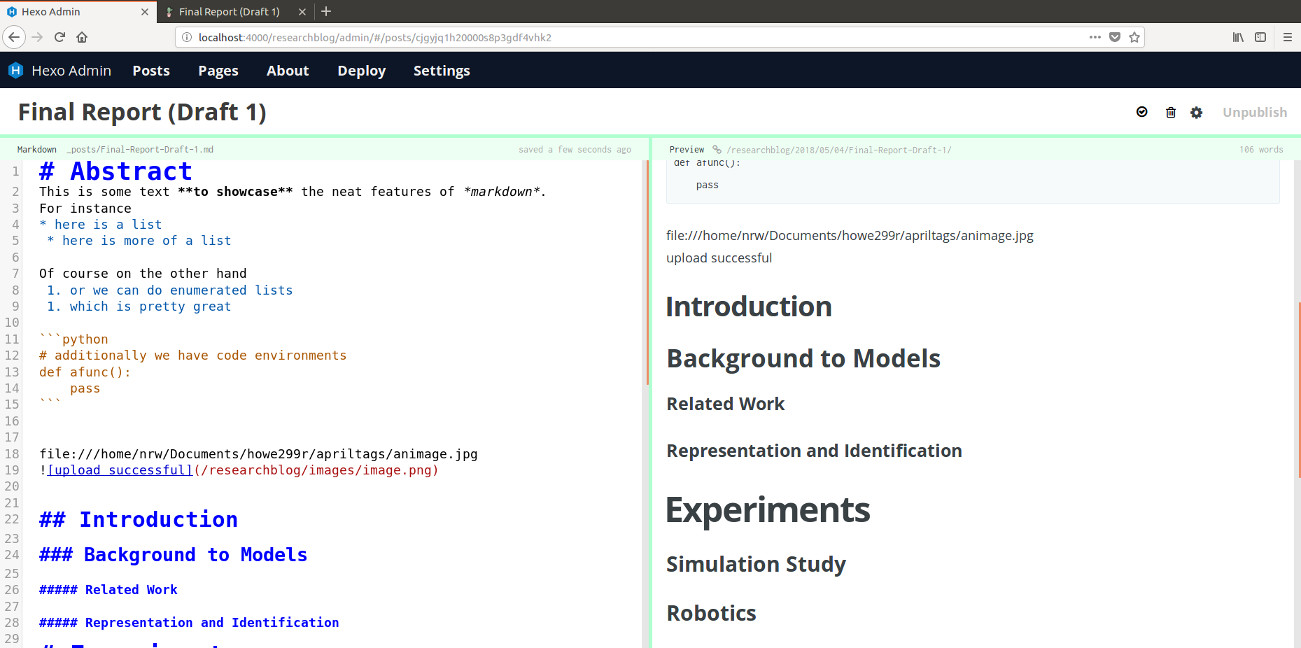
\includegraphics[width=0.8\textwidth]{images/misc/hexo_editor.jpg}
\caption{Hexo uses markdown, which is a nice simple markup language (although gets annoying really fast if you violate the KISS and try to do fancy things like include latex). It has a very nice GUI interface for editing posts. }
\end{figure}


\begin{figure}[H]
\centering
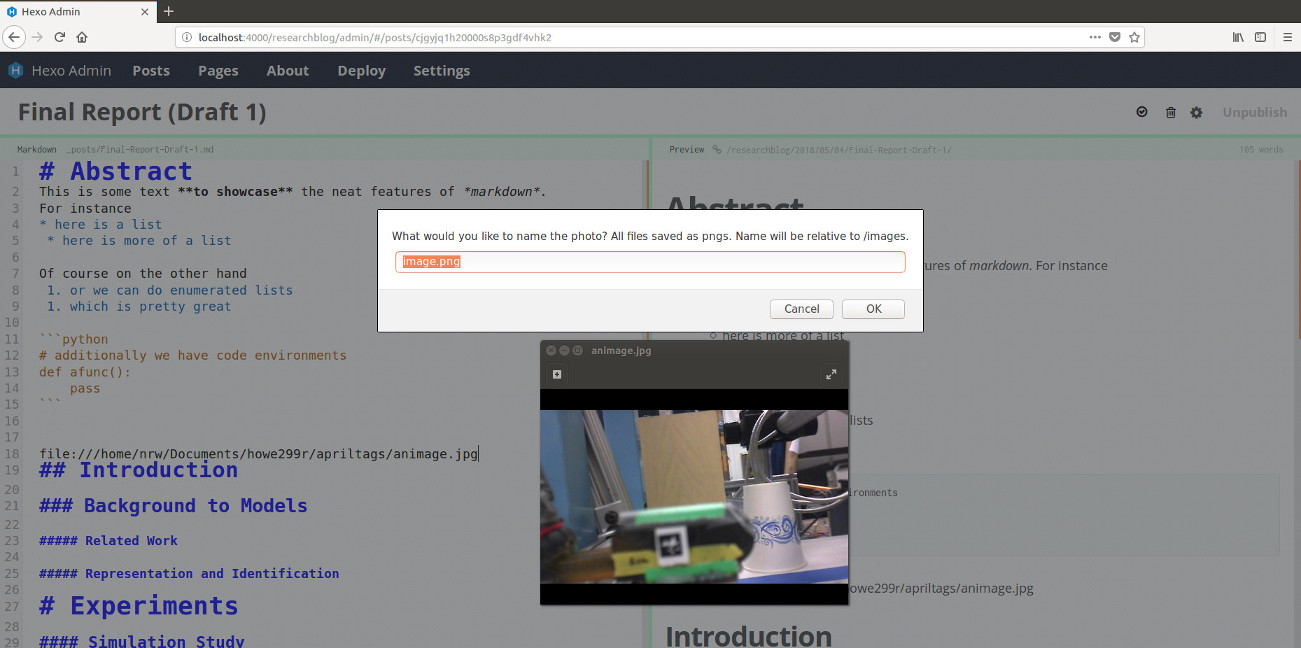
\includegraphics[width=0.9\textwidth]{images/misc/hexo_image.jpg}
\caption{The particular feature I was looking for was a drag-and-drop image manager. Although I
    could not get drag-and-drop plugin working, the default Hexo Admin editor allows you to copy
    paste (ctrl-c ctrl-v) pictures into the editor, and name them appropriately, which I considered
    good enough (and much better than the normal flat-file editor requirement of manually typing in
the file names and locations.}
\end{figure}

In particular, since I deal with many pictures for a given post, Hexo had a built-in configuration
to have a folder per post, which allowed for relatively easy image management.
\begin{lstlisting}
~$ vi _config.yml
    post_asset_folder: true  # REQUIRED even if you make folder by hand!!
\end{lstlisting}

I will be using Hexo in the future for my own projects (e.g. a portfolio website).


\section{Extra Graphs}
\label{appendix-graphs}

Here are a few graphs I didn't include for the sake of space, as they do not add
to the conversation.

\begin{figure}[H]
\centering
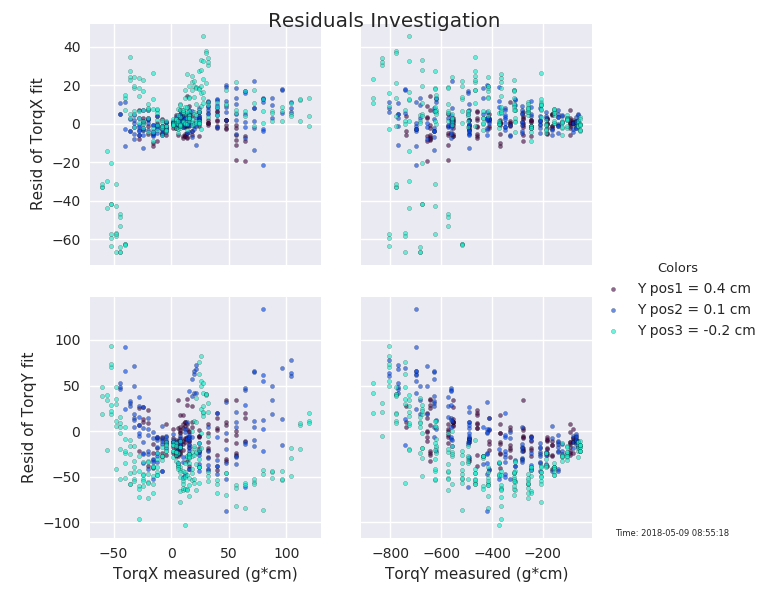
\includegraphics[width=1\textwidth]{images/round1/resids_Torq_coloredY}
\caption{A graph of the torque (linear fit) residuals vs. the measured torques.
The datapoints are shaded in by their Y position}
%\label{fig:figura1}
\end{figure}

\begin{figure}[H]
\centering
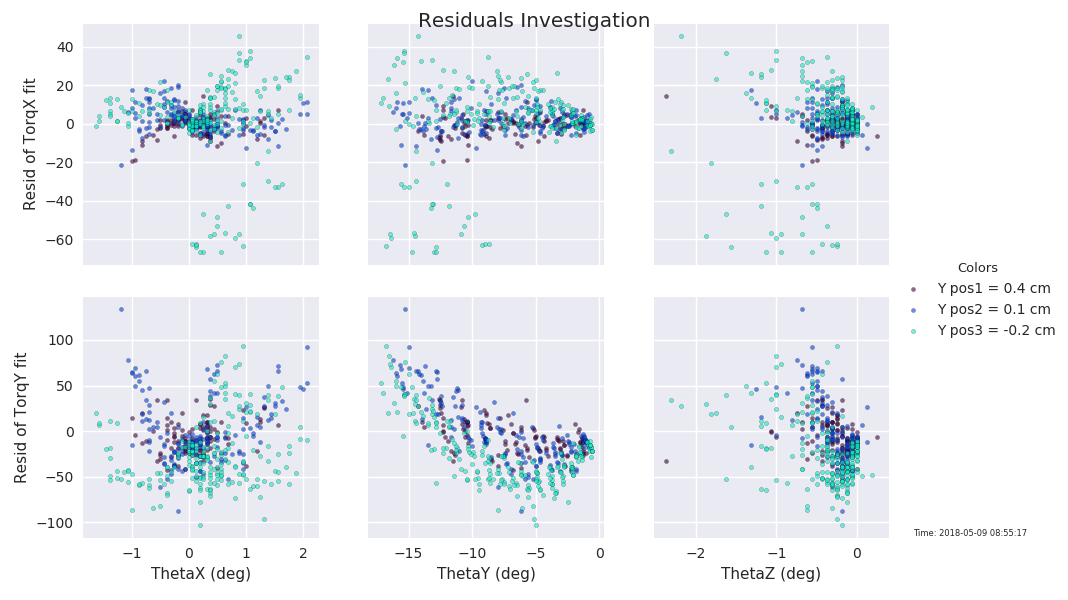
\includegraphics[width=1\textwidth]{images/round1/resids_Theta_coloredY.png}
\caption{A graph of the torque (linear fit) residuals vs. the measured angular
    deflections. The datapoints are shaded in by their Y position}
%\label{fig:figura1}
\end{figure}

\begin{figure}[H]
\centering
            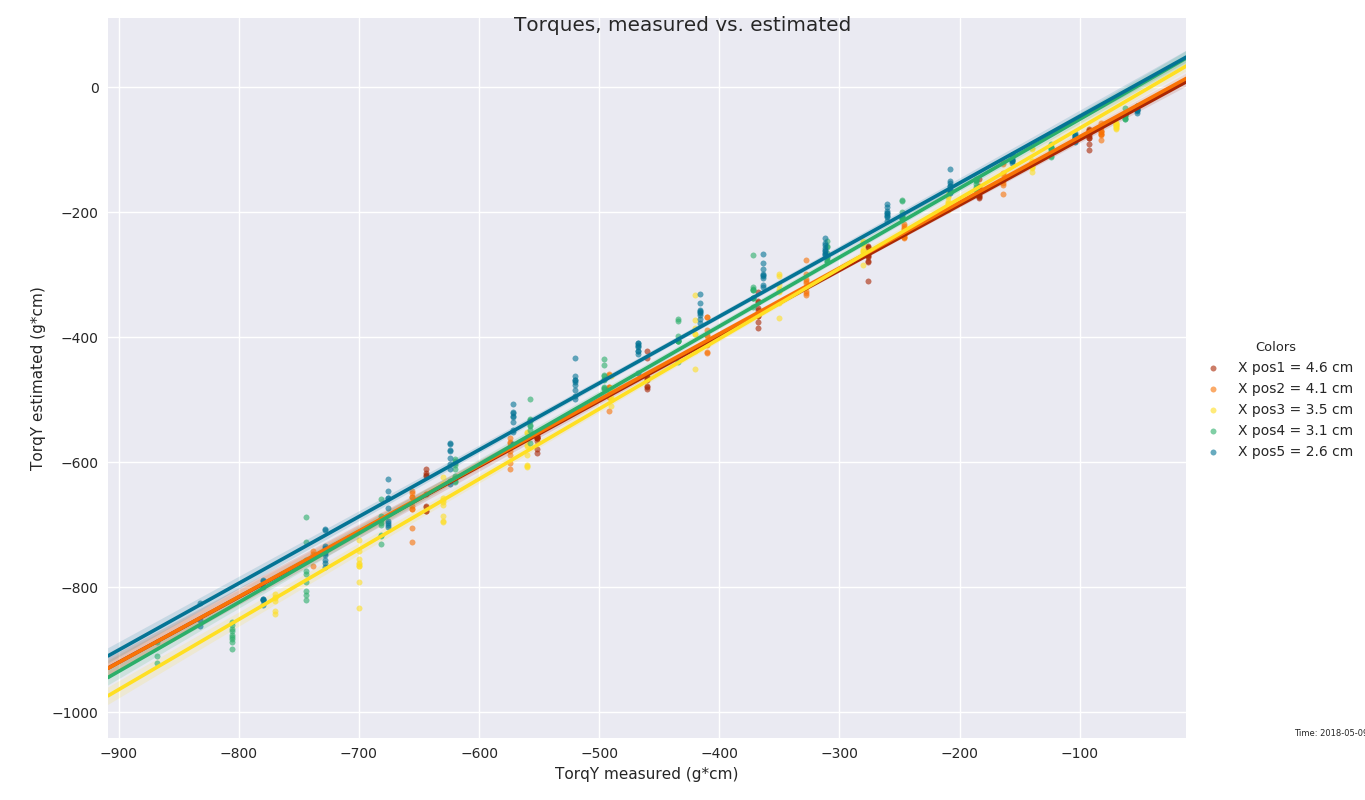
\includegraphics[width=0.9\textwidth]{images/round1/TorqY_Colors_X.png}%
            \caption{From the experiment with all 15 positions, we see that the Torque Y fit
            (measured vs estimated) is very clean.}
            \label{fig:yX}
\end{figure}

\newpage

\section{Additional Setup Pictures}
\label{appendix-setup}


\begin{figure}[H]
\centering
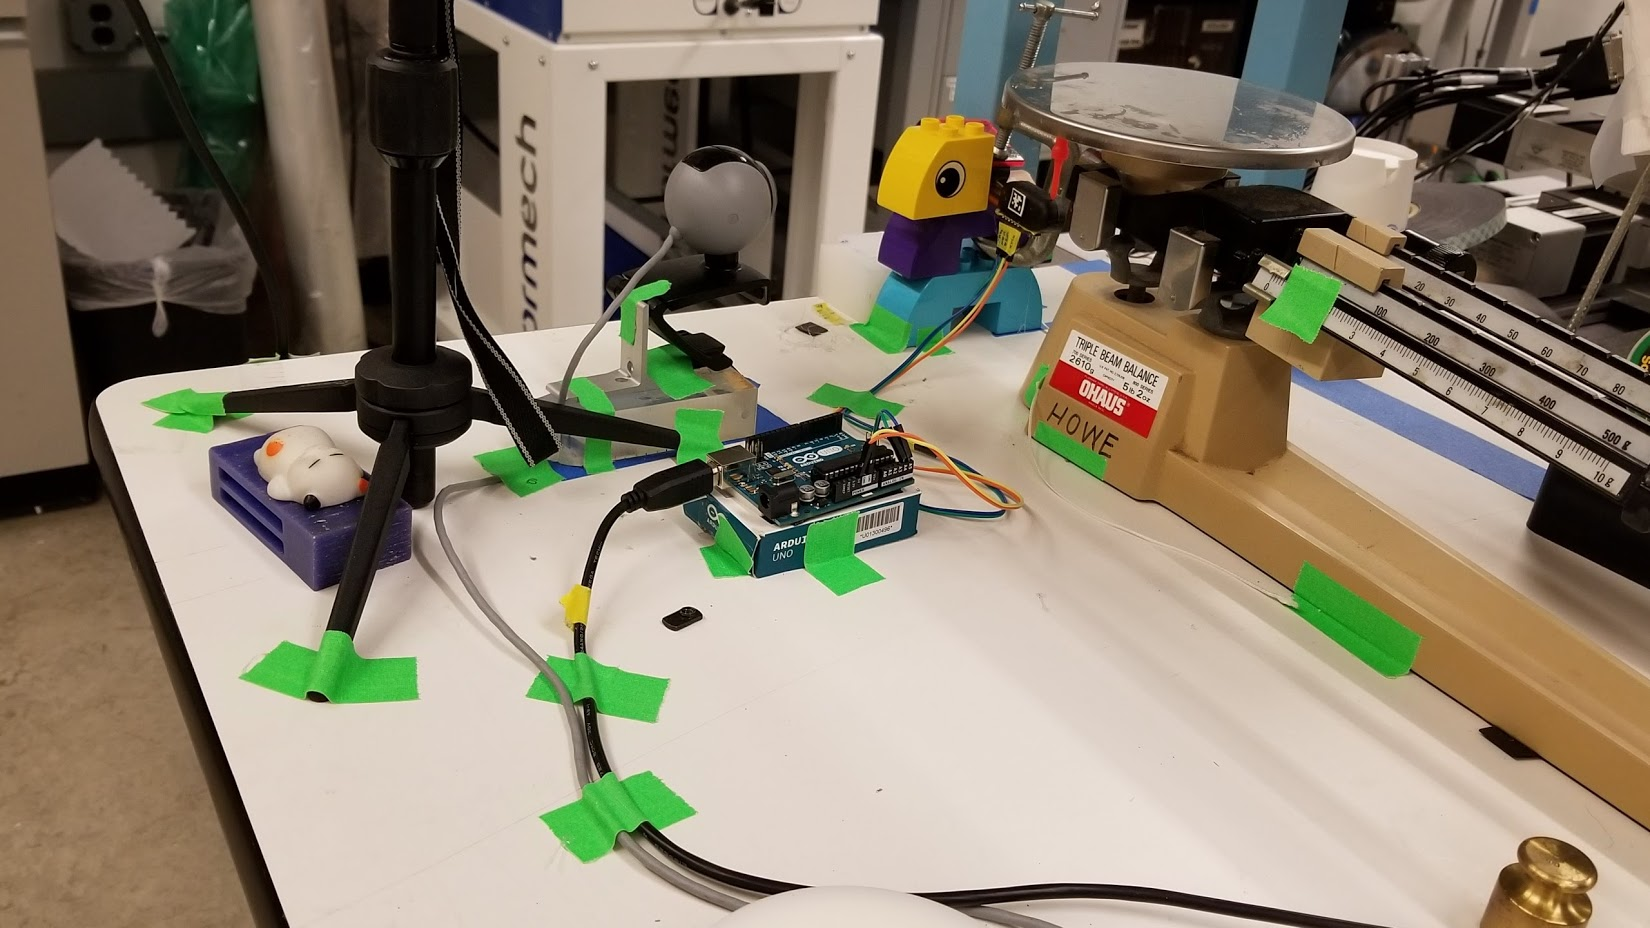
\includegraphics[width=0.9\textwidth]{images/setup/setup_closeup_tape.jpg}
\caption{Gratuitious amounts of tape were used as strain relief, to ensure that randomly bumping into or accidentally pulling on any of the power or sensor lines would not destroy the setup of equipment. Next time, I would just buy some white masking tape right away.
}
\end{figure}


\begin{figure}[H]
\centering
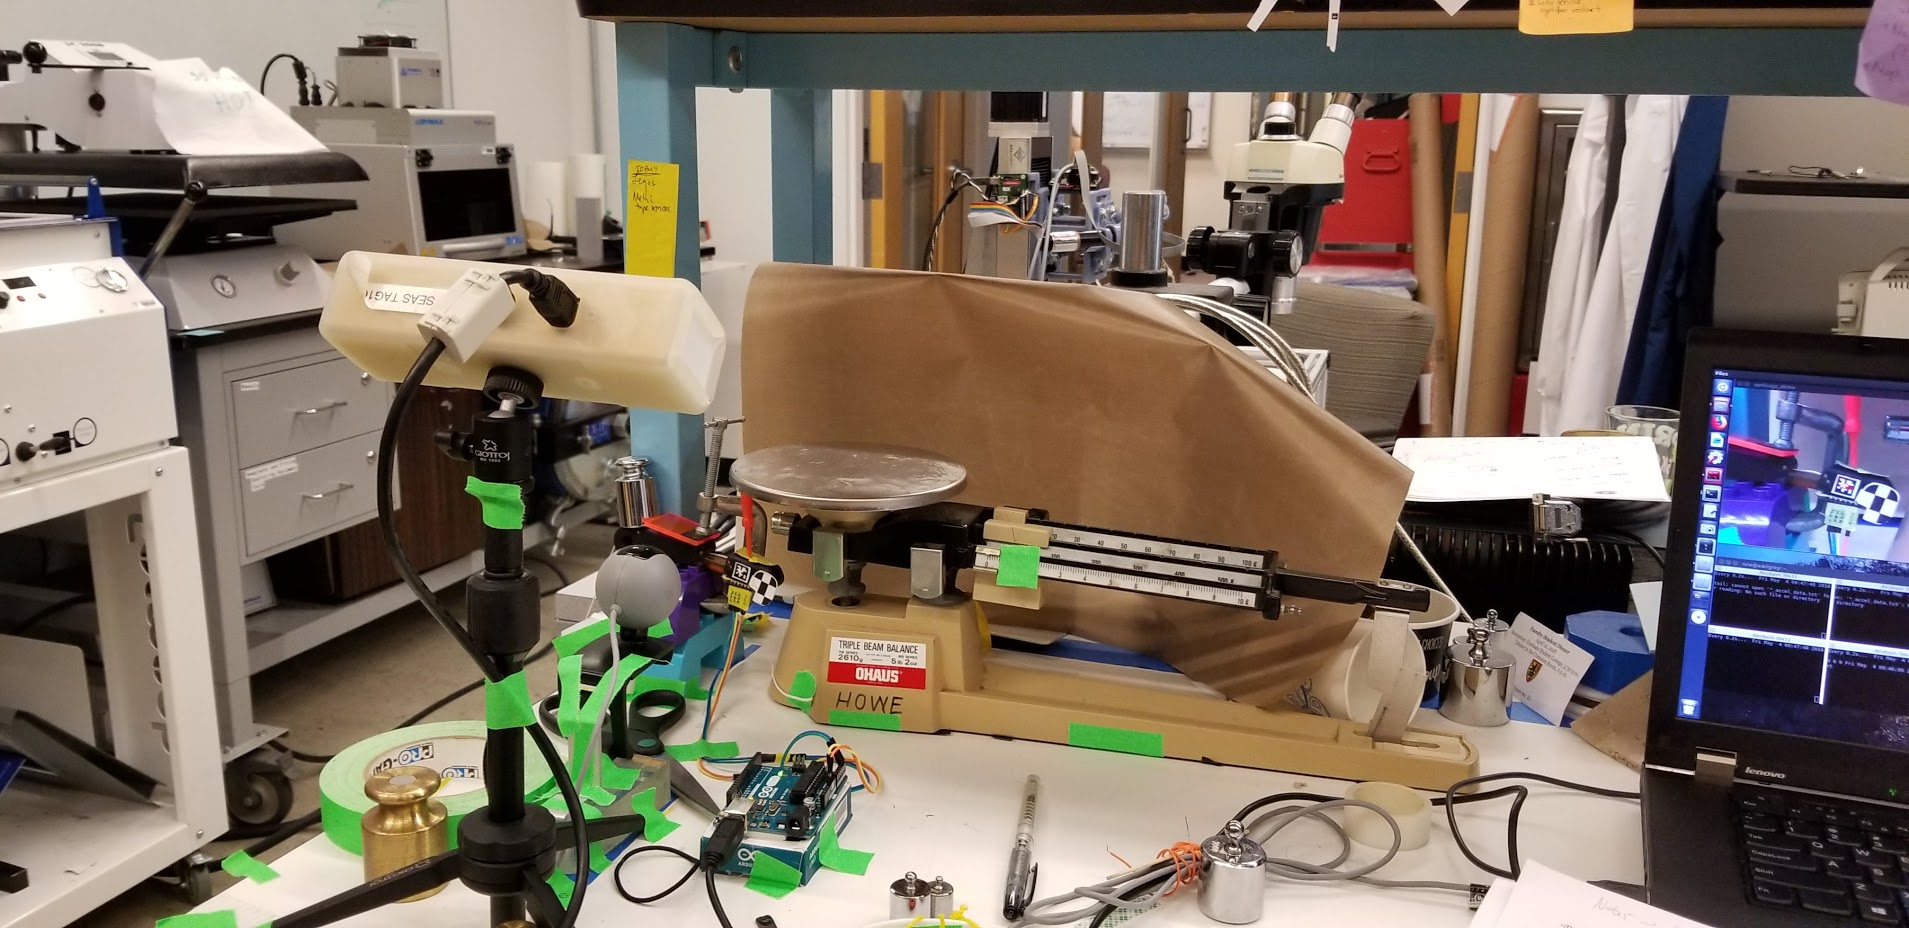
\includegraphics[width=1\textwidth]{images/setup/setup_overview.jpg}
\caption{An overview of the entire setup. This image is not included above as it's extremely messy and confusing, but it shows the relative placement of the microntracker, the webcam, the IMU, the arduino, and the triple beam balance.
}
\end{figure}

\section{Sensor Datasheets}
\label{appendix-sensors}

\begin{figure}[htbp]
    \centering 
        \subfloat[Note the single I2C address given, indicating this sensor has
        one fixed I2C address. Howevever, it has a "RST" line which can be used
        to turn off I2C communications for a chip, in effect acting as a chip
        select.
        ]{%
            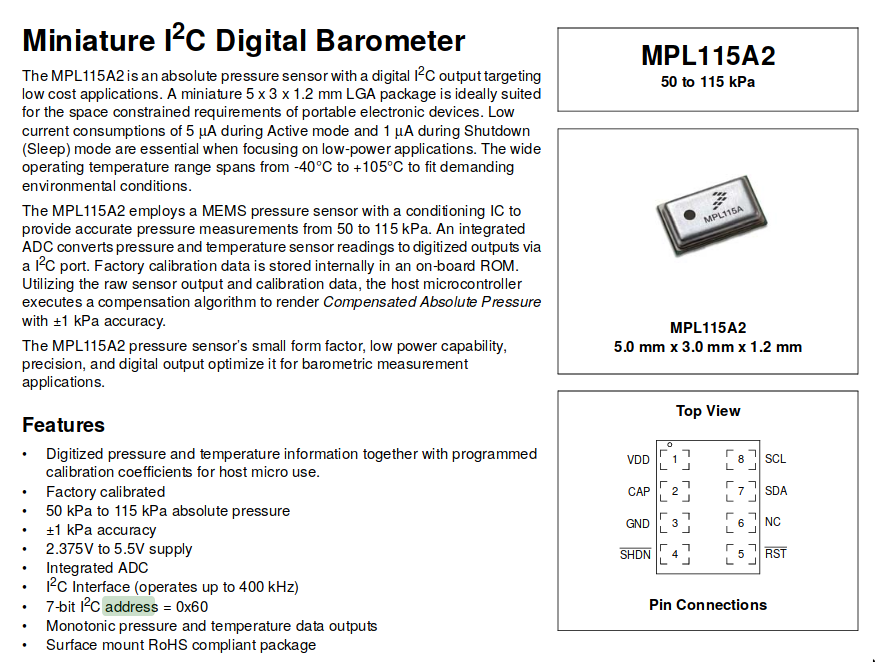
\includegraphics[width=0.8\linewidth]{images/sensor/MPL_i2c_address.png}%
        }\hfil % MUST be right above next figure
        \subfloat[Details about the BMP280 sensor, which is half the size of the
        MPL115 A2 sensor.
        ]{%
            \includegraphics[width=0.4\linewidth]{images/sensor/new_datasheet.png}%
        }\hfil
        \subfloat[An example of how to find out whether the I2C addresses are
        fixed for a given chip. Here we see that the BMP280 has 1 bit (2
        addresses) to choose from. 
        ]{%
            \includegraphics[width=0.5\textwidth]{images/sensor/BMP280_i2c_address.png}%
        }\hfil 
        \caption{Details about the two sensors: MPL115A2 on the current Takktile
            fingers in lab, and the new sensor I'm evaluating, the BMP280, which
        supports both I2C and SPI protocols.}
    \label{fig:i2c}
\end{figure}


With regards to the BMP280 sensors: I am using the Adafruit libraries with the
generic sensors.

Both breakouts have schematics available online.

\begin{figure}[H]
\centering
\includegraphics[width=0.4\textwidth]{images/sensor/generic_breakout_schematic.jpg}
\caption{Schematic for generic breakout. Note that aside form the sensor there
are just 2 resistors, 2 capacitors, and some header pins. Source: rainway87
seller on ebay}
%\label{fig:figura1}
\end{figure}


\begin{sidewaysfigure}
\centering
\includegraphics[width=\textwidth]{images/sensor/adafruit_breakout_schematic.png}
\caption{Schematic for Adafruit breakout. Source: adafruit.com}
%\label{fig:figura1}
\end{sidewaysfigure}
% References
%%
%% Following citation commands can be used in the body text:
%% Usage of \cite is as follows:
%%   \cite{key}         ==>>  [#]
%%   \cite[chap. 2]{key} ==>> [#, chap. 2]
%%

%% References with bibTeX database:

%\bibliographystyle{elsarticle-num}
%% \bibliographystyle{elsarticle-harv}
%% \bibliographystyle{elsarticle-num-names}
%% \bibliographystyle{model1a-num-names}
%% \bibliographystyle{model1b-num-names}
%% \bibliographystyle{model1c-num-names}
%% \bibliographystyle{model1-num-names}
%% \bibliographystyle{model2-names}
%% \bibliographystyle{model3a-num-names}
%% \bibliographystyle{model3-num-names}
%% \bibliographystyle{model4-names}
%% \bibliographystyle{model5-names}
%% \bibliographystyle{model6-num-names}

%\bibliography{sample}


\end{document}

%%
